\documentclass{article}

\counterwithin{figure}{section}
\counterwithin{equation}{section}

\newcommand{\sign}{\operatorname{sign}}
%\newcommand{\trans}{^{\mkern-1.5mu\mathsf{T}}}
%\newcommand{\hermit}{^\dagger}
%\newcommand{\ident}{\mathds{1}}
%\newcommand{\pdvconst}[4][]{\left(\pdv[#1]{#2}{#3}\right)_{\!\!\!{#4}}}
%\newcommand{\dvat}[4][]{\dv[#1]{#2}{#3}\Biggr|_{#4}}
%\newcommand{\pdvat}[4][]{\pdv[#1]{#2}{#3}\Biggr|_{#4}}
%\newcommand{\pdvsec}[3]{\frac{\partial^2{#1}}{\partial{#2}\partial{#3}}}
%\newcommand{\pdvsecat}[4]{\pdvsec{#1}{#2}{#3}\Biggr|_{#4}}

\title{Linear Algebra and Several Variable Calculus}
\author{Willoughby Seago}
\date{September 17, 2019}
\usepackage{NotesPackage}
\usepackage{csquotes}
\usepackage{listings}
\usetikzlibrary{calc}

\renewcommand{\grad}{\nabla}
\renewcommand{\div}{\nabla\cdot}
\renewcommand{\curl}{\nabla\times}

\newcommand{\notesVersion}{1.0}
\newcommand{\notesDate}{04/01/2021}

\begin{document}
    \maketitle
    These are my notes for the \textit{linear algebra and several variable calculus (LASVC)} course from the University of Edinburgh as part of the second year of the theoretical physics degree.
    When I took this course in the 2019/20 academic year it was taught by Professor Philip Clark\footnote{\url{https://www.ph.ed.ac.uk/people/philip-clark}}.
    These notes are based on the lectures delivered as part of this course, and the notes provided as part of this course.
    The content within is correct to the best of my knowledge but if you find a mistake or just disagree with something or think it could be improved please let me know.
    
    These notes were produced using \LaTeX\footnote{\url{https://www.latex-project.org/}}.
    Graphs where plotted using Python\footnote{\url{https://www.python.org/}}, Matplotlib\footnote{\url{https://matplotlib.org/}}, NumPy\footnote{\url{https://numpy.org/}}, and SciPy\footnote{\url{https://scipy.org/scipylib/}}.
    Diagrams were drawn with tikz\footnote{\url{https://www.ctan.org/pkg/pgf}}.
    Some images were taken from the lecture notes provided.
    
    This is version \notesVersion~of these notes, which is up to date as of \notesDate.
    \begin{flushright}
        Willoughby Seago
        
        s1824487@ed.ac.uk
    \end{flushright}
    \clearpage
    \tableofcontents
    \listoffigures
    \clearpage
    
    \section{Basic Vectors}
    A vector \(\vv a\) has magnitude, \(|\vv a|=a\), and direction.
    
    A binary operator \(*\) acting on elements \(a\) and \(b\) is commutative if \(a*b=b*a\). 
    The same operator is said to be anti-commutative if instead \(a*b=-b*a\).
    
    Vector addition is commutative as \(\vv a + \vv b = \vv b + \vv a\).
    
    The vector \(c\vv a\) for \(c > 0\) points in the same direction as \(\vv a\) and has magnitude \(ca\). 
    For \(c < 0\) the vector \(c\vv a\) points in the opposite direction to \(\vv a\) and has magnitude \(-ca\).
    
    A unit vector is any vector with magnitude 1. It is denoted as \(\vh a\) where \(\vh a\) points in the same direction as \(\vv a\) and has magnitude 1.
    The unit direction in the direction of \(\vh a\) can be calculated as \(\vh a = \vv a / a\)
    
    The scalar (dot) product between two vectors \(\vv a\) and \(\vv b\) is defined as \(\vv a\cdot\vv b = ab\cos\vartheta\) where \(\vartheta\) is the angle between the vectors.
    
    \section{More Basic Vectors}
    A point \(P\) on a line in direction \(\vv a\) can be given as \(\overrightarrow{OP}=\lambda\vv a\). For this reason a line is a 1D vector space.
    
    A point \(P\) on a plane containing linearly independent vectors \(\vv a\) and \(\vv b\) can be given as \(\overrightarrow{OP} = \lambda a + \mu b\). For this reason a plane is a 2D vector space.
    
    For 2D and up it is easier to work with orthogonal vectors as basis vectors as this keeps the scalar coefficients as low as possible. If we have two vectors \(\vv a\) and \(\vv b\) that are linearly independent and a third vector \(\vv c = \vv a + \vv b\) then we can perform a process called orthonormalisation to find a set of orthonormal vectors.
    \begin{center}
        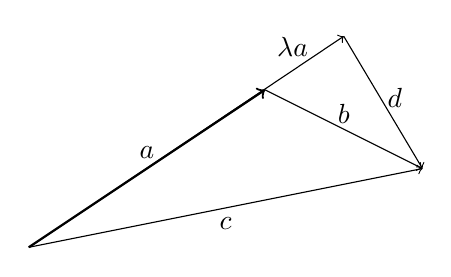
\begin{tikzpicture}
            %\draw[lightgray] (0, 0) grid (5, 5);
            \draw[->, thick] (0, 0) -- (3, 2);
            \draw[->] (3, 2) -- (5, 1);
            \draw[->] (0, 0) -- (5, 1);
            \node at (1.5, 1.2) {\(\vv a\)};
            \node at (4, 1.7) {\(\vv b\)};
            \node at (2.5, 0.3) {\(\vv c\)};
            \draw[->] (0, 0) -- (4, 2.68);
            \draw[->] (4, 2.68) -- (5, 1);
            \node at (3.35, 2.55) {\(\lambda\vh a\)};
            \node at (4.65, 1.9) {\(\vv d\)};
        \end{tikzpicture}
    \end{center}
    \(\vv d\) is perpendicular to \(\vv a\)
    
    \begin{align*}
        \vv c &= \vv a + \vv b\\
        \vv c &= \lambda\vh a + \vv d\\
        \vv c\cdot\vh a &= \lambda\underbrace{\vh a\cdot\vh a}_{=1}+\underbrace{\vv d\cdot\vh a}_{=0}\\
        \lambda &=\vv c\cdot \vh a\\
        \vv d &= \vv c - \lambda\vh a\\
        \vv d &= \vv c - (\vv c\cdot\vh a)\vh a
    \end{align*}
    
    Given a plane containing linearly independent vectors \(\vv a\) and \(\vv b\) any vector \(\vv c\) can be decomposed into an in-plane (transverse) component \(\vv v_t\) and a normal component \(\vv v_n\). We assume here that the normal unit vector \(\vh n\) for the plane is known as this is the most common way to define a plane. Otherwise this can be calculated as \(\vv a\times\vv b/|\vv a\times\vv b|\).
    \begin{align*}
        \vv c &= \vv v_t + \vv v_n\\
        \vv c &= \vv v_t + \lambda\vh n\\
        \vv c\cdot\vh n &= \vv v_t\cdot\vh n + \lambda\vh n\cdot\vh n\\
        \vv c\cdot\vh n &= 0 + \lambda\\
        \vv c\cdot\vh n &= \lambda\\
        \vv v_t &= \vv c -(\vv c\cdot\vh n)\vh n
    \end{align*}
    
    The cross product of \(\vv a\) and \(\vv b\) is defined as the vector normal to both \(\vv a\) and \(\vv b\) following the right hand rule and with magnitude \(|\vv a\times\vv b|=ab\sin\vartheta\).
    
    \section{Orthonormal Basis Sets}
    \subsection{Equation of a Line}
    A line is in direction \(\vv a\) and point \(\vv p\) lies on the line. 
    The position of a general point \(\vv r\) on the line is given by
    \[\vv r = \vv p +\lambda \vv a\]
    \[\vv r\times\vv a=\vv a\times\vv p+\lambda\vv a\times\vv a\]
    \[(\vv r-\vv p)\times\vv a=\vv 0\]
    
    This can be understood as \(\vv p\) taking you from the origin to the line and \(\lambda\vv a\) taking you along the line to the desired point.
    
    \begin{figure}[ht]
        \centering
        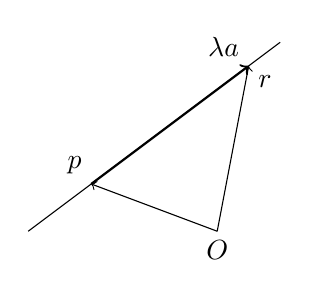
\begin{tikzpicture}[scale=0.8]
            %\draw[lightgray] (0, 0) grid (5, 5);
            \draw (0, 0) -- (4, 3);
            \draw[->] (3, 0) -- (1, 0.75);
            \node[below] at (3, 0) {\(O\)};
            \node[above left] at (1, 0.75) {\(\vv p\)};
            \draw [->, thick] (1, 0.75) -- (3.5, 2.625);
            \node[above left] at (3.5, 2.625) {\(\lambda\vv a\)};
            \draw[->] (3, 0) -- (3.5, 2.625);
            \node[below right] at (3.5, 2.625) {\(\vv r\)};
        \end{tikzpicture}
        \caption{A point on the line \(\vv r = \vv p + \lambda \vv a\)}
    \end{figure}

    \subsection{Equation of a Plane}
    For two vectors \(\vv a\) and \(\vv b\) in a plane normal to \(\vh n\) with non-zero angle between \(\vv a\) and \(\vv b\) and a point on the plane \(\vv p\) the equation of the plane can be given as:
    \[\vv r = \vv p +\lambda\vv a + \mu\vv b\]
    \[\vv r - \vv p= \lambda\vv a + \mu\vv b\]
    \[(\vv r - \vv p)\cdot\vh n = \lambda\vv a\cdot\vh n + \mu\vv b\cdot\vh n\]
    \begin{equation}\label{eq:(r-p).n=0}
        (\vv r - \vv p)\cdot\vh n = 0
    \end{equation}
    This can be generalised to any \(d\)-dimensional space with \(d\)-dimensional normal \(\vh n\), two \(d\)-dimensional points \(\vv p\) and \(\vv r\) will satisfy equation~\ref{eq:(r-p).n=0}.
    
    \subsection{Orthonormal Basis Set}
    An orthonormal basis set is a set of mutually perpendicular unit vectors, usually denoted \(\ve i\) where \(i\in\bb N\), \(|\ve i|=1\) and if \(i \ne j\) then \(\ve i\cdot\ve j=0\). 
    A d-dimensional vector \(\vv a\) can be decomposed into components of this basis set
    \[\vv a=a_1\ve 1 + a_2\ve 2 +\dotsb+a_d\ve d\]
    The coefficient of \(\ve i\) can be found using the dot product
    \[\vv a\cdot\ve i=a_i\]
    since this goes to 0 for all terms not including \(\ve i\) and \(\ve i\cdot \ve i = 1\).
    
    There is more than one orthonormal basis set
    
    \begin{figure}[ht]
        \centering
        \begin{tikzpicture}
            \draw[->] (0, 0) -- (2, 0);
            \draw[->] (0, 0) -- (0, 2);
            \node[right] at (2, 0) {\(\ve 1\)};
            \node[above] at (0, 2) {\(\ve 2\)};
            \draw[->] (0, 0) -- (1.5, 1.5);
            \node[above right] at (1.5, 1.5) {\(\vv a\)};
            
            \begin{scope}[xshift=3cm]
                \begin{scope}[rotate=-30]
                    \draw[->] (0, 0) -- (2, 0);
                    \draw[->] (0, 0) -- (0, 2);
                    \node[right] at (2, 0) {\(\ve 1'\)};
                    \node[above] at (0, 2) {\(\ve 2'\)};
                \end{scope}
                \draw[->] (0, 0) -- (1.5, 1.5);
                \node[above right] at (1.5, 1.5) {\(\vv a\)};
            \end{scope}
        \end{tikzpicture}
        \caption{Multiple orthonormal basis sets}
        \label{fig:multiple orthonormal basis sets}
    \end{figure}
    
    \(\vv a\) in figure~\ref{fig:multiple orthonormal basis sets} can be given as:
    \[\vv a = a_1\ve 1 + a_2\ve 2 = a_1'\ve 1' + a_2'\ve 2'\]
    or in terms of column vectors
    \[
        \vv a = 
        \begin{pmatrix}
            a_1 \\ a_2
        \end{pmatrix}_B
        \qquad
        \vv a =
        \begin{pmatrix}
            a_1' \\ a_2'
        \end{pmatrix}_{B'}
    \]
    Where the subscript \(B\) or \(B'\) tells us the basis we are in.
    Note that in general
    \[
        \begin{pmatrix}
        a_1 \\ a_2
        \end{pmatrix}_B
        \ne
        \begin{pmatrix}
        a_1' \\ a_2'
        \end{pmatrix}_{B'}
    \]
    as the basis vectors aren't included in this representation in the way that they are in \(\vv a = a_i\ve i\).
    
    \subsection{Linear Independence}
    A set of \(d\) vectors spans a \(d\)-dimensional space if the vectors are linearly independent. 
    
    A set of \(d\) vectors \(\vv v_1, \vv v_2,\dotsc, \vv v_d\) is linearly independent if and only if \(c_1 = c_2 = \dotsb = c_d = 0\) is the only solution to
    \[c_1\vv v_1 + c_2\vv v_2 + \dotsb c_d\vv v_d = 0\]
    
    For example two co-linear vectors \(\vv a\) and \(\vv b\) aren't linearly independent as \(\vv a = \lambda\vv b\) so \(\vv a - \lambda\vv b = 0\) \(\A\vv a\) and \(\vv b\).
    
    A 3-dimensional orthonormal basis set is right handed if
    \[\ve 1\times\ve 2 = \ve 3 \qquad \ve 2\times\ve 3 = \ve 1 \qquad \ve 2\times\ve 1 = \ve 2\]
    
    \section{Orthonormalisation}
    
    For two \(n\)-dimensional vectors \(\vv a\) and \(\vv b\) we can write them as sums
    \[\sum_{i=1}^{n}a_i\ve i \qquad \& \qquad \sum_{j=1}^{n}b_j\ve j\]
    We define the Kronecker delta \(\delta\) as
    \[
        \delta_{ij} = \left\{
        \begin{array}{cc}
            1 & i = j\\
            0 & i \ne j
        \end{array}
        \right.
    \]
    This allows us to write the dot product for two unit vectors \(\ve i\) and \(\vv j\) as
    \[\ve i\cdot \ve j = \delta_{ij}\]
    We can use this to write the dot product for \(\vv a\) and \(\vv b\) as sums for which we will use the notation \(\sum_i\) to indicate that we are summing over all values of \(i\).
    \begin{align*}
        \vv a\cdot\vv b &= \left(\sum_i a_i\ve i\right)\cdot\left(\sum_j a_j\ve j\right)\\
        &= \sum_i\sum_ja_ib_j\ve i\cdot \ve j\\
        &= \sum_i\sum_j\delta_{ij}a_ib_j\\
        \intertext{Since all terms have a factor of \(\delta_{ij}\) any term where \(i\ne j\) goes to 0 so we can sum over only one index by setting \(i = j\)}
        &= \sum_i a_ib_i
    \end{align*}
    
    \subsection{Creating orthonormal basis sets}
    In 1-dimension if we have a vector \(\vv a\) we can just use \(\ve 1 = \vh a = \vv a/a\) as a basis vector.
    
    In 2-dimensions if we have linearly independent vectors \(\vv a\) and \(\vv b\) we start by using \(\ve 1 = \vh a = \vv a/a\).
    We then need to find a second perpendicular unit vector to this. We do this by taking \(\vv b\) and subtracting the component in the direction of \(\vv a\) to construct a vector \(\vv c\) perpendicular to \(\ve 1\).
    \[\vv c = \vv b - (\vv b\cdot\vh a)\vh a\]
    We can then set our second basis vector to \(\ve 2 = \vh c = \vv c/c\), written in terms of \(\vv a\) and \(\vv b\) this is:
    \[\ve 2 = \frac{\vv b - (\vv b\cdot\vh a)\vh a}{|\vv b - (\vv b\cdot\vh a)\vh a|}\]
    Note that if \(\vv a\) and \(\vv b\) aren't linearly independent then \(\vartheta = 0\) and 
    \begin{align*}
        \vv c &= \vv b - (\vv b\cdot\vh a)\vh a\\
        &= \vv b - b\cos(\vartheta)\vh a\\
        &= \vv b - b\vh a\\
        \intertext{Since \(\vv a\) and \(\vv b\) are in the same direction \(\vv b = b\vh a\)}
        &= \vv b - \vv b\\
        &= 0
    \end{align*}
    This process is called Gram-Schmidt orthonormalisation
    
    \subsection{Gram-Schmidt Orthonormalisation}
    We can iterate over this process to find \(\ve 3\) if we have some vector \(\vv d\) which is linearly independent to \(\vv a\) and \(\vv b\).
    \[\ve 3 = \frac{\vv d - (\vv d\cdot\ve 1)\ve 1 - (\vv d\cdot\ve 2)\ve 2}{|\vv d - (\vv d\cdot\ve 1)\ve 1 - (\vv d\cdot\ve 2)\ve 2|}\]
    
    For the n\(^\text{th}\) step of this process:
    \begin{itemize}
        \item Have \(n-1\) unit vectors \(\ve 1, \ve 2,\dotsc,\ve{n-1}\)
        \item Given an n\(^\text{th}\) vector \(\vv v_n\), which is linearly independent to these unit vectors, we can find a vector \(\vv v_n'\):
        \[\vv v_n' = \vv v_n - (\vv v_n\cdot \ve 1)\ve 1 - (\vv v_n\cdot\ve 2)\ve 2-\dotsb-(\vv v_n\cdot\ve{n-1})\ve{n-1}\]
        \item Normalise this vector to get
        \[\ve n = \frac{\vv v_n'}{v_n'}\]
    \end{itemize}
    You run out of vectors when \(\vv v_n\) can be written as \(\vv v_n = a_1\vv v_1 + a_2\vv v_2+\dotsc a_{n-1}\vv v_{n-1}\)
    
    \subsection{Triple Products}
    The area of a parallelogram with adjacent sides \(\vv a\) and \(\vv b\) is given by \(|\vv a\times\vv b|\).
    
    The volume of a parallelepiped constructed from the above parallelogram with a third side \(\vv c\) is \(|(\vv a\times\vv b)\cdot c|\). This is called the scalar triple product.
    
    The vector triple product is
    \[\vv a\times(\vv b\times\vv c) = \vv b(\vv a\cdot\vv c) - \vv c(\vv a\cdot\vv b)\]
    
    \example
    An associative operator \(\circ\) satisfies \(A\circ(B\circ C) = (A\circ B)\circ C\). Is the cross product \(\times\) associative?
    
    We can show that it isn't using the vector triple product. First we use the anti-commutativity of the cross product
    \[(\vv a\times\vv b)\times\vv c = -\vv c\times(\vv a\times\vv b)\]
    \begin{equation}
        =\vv a(\vv c\cdot\vv b) - \vv b(\vv c\cdot\vv a)\label{(axb)xc}
    \end{equation}
    \begin{equation}
        \vv a\times(\vv b\times\vv c) = \vv b(\vv a\cdot\vv c) - \vv c(\vv a\cdot\vv b)\label{ax(bxc)}
    \end{equation}
    
    These are clearly different as equation~\ref{(axb)xc} has components in the \(\vv a\) and \(\vv b\) directions where as equation~\ref{ax(bxc)} has components in the \(\vv b\) and \(\vv c\) directions.

    \subsection{Levi-Civita Symbol}
    The Levi-Civita symbol \(\varepsilon\) is defined as
    \[
        \varepsilon_{ijk} = \left\{
        \begin{array}{cc}
            +1 & ijk = 123, 312, 231\\
            -1 & ijk = 132, 321, 213\\
            0  & i=j, j=k, i=k
        \end{array}
        \right.
    \]
    For example \(\varepsilon_{312}=1\), \(\varepsilon_{213}=-1\) and \(\varepsilon_{121}=0\).
    
    In more dimensions \(\varepsilon_{i_1i_2\dotso i_n}\) is defined as \(1\) if \(i_1i_2\dots i_n\) is an even permutation (requires an even number of two element swaps to return to \(12\dotso n\)), \(-1\) if it is an odd permutation (requires an odd number of swaps to return to \(12\dotso n\)) or 0 if there are repeated indices.
    
    We can use this to write the cross product in a more concise way
    \[(\vv a\times\vv b)_i = (\vv a\times\vv b)\cdot\ve i=\sum_{j=1}^{3}\sum_{k=1}^{3}\varepsilon_{ijk}a_jb_k\]
    \[\vv a\times\vv b = \sum_i\sum_j\sum_k\varepsilon_{ijk}\ve ia_jb_k\]
    
    \section{Matrices}
    
    \subsection{More on the Scalar Triple Product}
    If \(\vv a\), \(\vv b\) and \(\vv c\) aren't linearly independent then their scalar triple product \(\vv a\cdot(\vv b\times\vv c) = 0\). 
    This means that the scalar triple product can be used to test for linear independence.
    
    Consider the parity transform \(\ve i' = -\ve i\). This changes the parity of the coordinate system.
    \[\vv a\cdot(\vv b\times\vv c) = -\vv a\cdot(-\vv b\times-\vv c) = -\vv a\cdot(\vv b\times\vv c)\]
    So the sign of the scalar triple product changes under a parity change. For this reason we call the scalar triple product a pseudo-scalar
    
    \subsection{Matrices}
    Consider a 2-dimensional vector \(\vv a\). It can be written in multiple different ways:
    \[\vv a = a_1\ve 1 + a_2\ve 2\]
    \[\vv a = a_1'\ve 1' + a_2'\ve 2'\]
    Where \(\{\ve 1, \ve 2\}\) and \(\{\ve 1, \ve 2\}\) are orthonormal basis sets.
    Our aim is to find the components \(a_i'\).
    In general we can find the \(\ve i\) component by dotting with \(\ve i\):
    \[\vv a\cdot\ve i = a_1'(\ve i\cdot\ve 1') + a_2'(\ve i\cdot\ve 2')\]
    For an \(n\)-dimensional vector \(\vv a\)
    \[a_i' = \sum_{j = 1}^{n}a_j(\ve i\cdot\ve j')\]
    \(a_i'\) is a weighted sum of the components in the original basis set. We can write this transform as
    \[
        \begin{pmatrix}
            a_1' \\ a_2' \\ \vdots \\ a_n'
        \end{pmatrix}
        = P
        \begin{pmatrix}
            a_1 \\ a_2 \\ \vdots \\ a_n
        \end{pmatrix}
    \]
    \(P\) is an \(n\times n\) array of numbers and specifies the weights. \(P_{ij}\) is the element of \(P\) at row \(i\) and column \(j\).
    We can write \(P\) out as an array of dot products
    \[
        \begin{pmatrix}
            a_1' \\ a_2' \\ \vdots \\ a_n'
        \end{pmatrix}
        =
        \begin{pmatrix}
            \ve 1'\cdot \ve 1 & \ve 1'\cdot \ve 2 & \cdots & \ve 1'\cdot \ve n\\
            \ve 2'\cdot \ve 1 & \ve 2'\cdot \ve 2 & \cdots & \ve 2'\cdot \ve n\\
            \vdots & \vdots & \ddots & \vdots\\
            \ve n'\cdot \ve 1 & \ve n'\cdot \ve 2 & \cdots & \ve n'\cdot \ve n
        \end{pmatrix}
        \begin{pmatrix}
            a_1 \\ a_2 \\ \vdots \\ a_n
        \end{pmatrix}
    \]
    A matrix provides a way to define a linear transformation. 
    It doesn't have a physical meaning itself.
    
    For matrices \(A\) and \(B\) the matrix product \(AB\) is defined if and only if the number of columns in \(A\) is the same as the number of rows in \(B\).
    The element \(AB_{ij}\) is the dot product of row \(i\) of \(A\) and column \(j\) of \(B\).
    Doing transformation \(A\) and then \(B\) is equivalent to doing the transformation \(BA\).
    In general \(AB \ne BA\).
    
    \section{Orthogonal Matrices}
    The identity matrix \(\ident\) is the matrix \([\ident]_{ij} = \delta_{ij}\)
    
    The inverse of matrix \(M\) is defined as the matrix \(M^{-1}\) such that
    \[MM^{-1} = M^{-1}M = \ident\]
    The transpose of a matrix \(M\) is defined as the matrix \(M\trans\) that results from swapping the rows and columns of \(M\)
    \[[M\trans]_{ij} = M_{ji}\]
    
    A passive transformation is one where the vector that it acts on is unaffected but the basis changes.
    
    An example of this is a rotation, anticlockwise, about the origin, by an angle of \(\vartheta\) as shown if figure \ref{fig:rotation}
    \begin{figure}[ht]
        \centering
        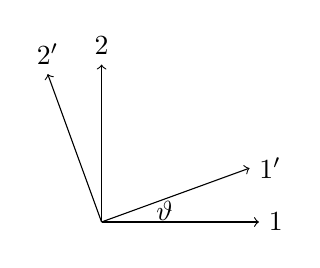
\begin{tikzpicture}
            \draw[->] (0, 0) -- (2, 0) node[right] at (2, 0) {\(\ve 1\)};
            \draw[->] (0, 0) -- (0, 2) node[above] at (0, 2) {\(\ve 2\)};
            
            \begin{scope}[rotate around={20:(0, 0)}]
                \draw[->] (0, 0) -- (2, 0) node[right] at (2, 0) {\(\ve 1'\)};
                \draw[->] (0, 0) -- (0, 2) node[above] at (0, 2) {\(\ve 2'\)};
            \end{scope}
            \node at (0.8, 0.14) {\(\vartheta\)};
        \end{tikzpicture}
        \caption{Rotation of basis}
        \label{fig:rotation}
    \end{figure}
    By projecting the the new basis vectors onto the old ones we can calculate the transformation matrix \(R(\vartheta)\):
    \[
        P = 
        \begin{pmatrix}
            \ve 1'\cdot \ve 1 & \ve 1'\cdot \ve 2\\
            \ve 2'\cdot \ve 1 & \ve 2'\cdot \ve 2
        \end{pmatrix}
        =
        \begin{pmatrix}
            \cos\vartheta & \sin\vartheta\\
            -\sin\vartheta & \cos\vartheta
        \end{pmatrix}
    \]
    The inverse of a rotation is a rotation by the same amount in the opposite direction so in this case \(R(-\vartheta)\)
    \[
        R^{-1}(\vartheta)
        =
        \begin{pmatrix}
            \cos-\vartheta & \sin-\vartheta\\
            -\sin-\vartheta & \cos-\vartheta
        \end{pmatrix}
        =
        \begin{pmatrix}
            \cos\vartheta & -\sin\vartheta\\
            \sin\vartheta & \cos\vartheta
        \end{pmatrix}
    \]
    From this we can see that
    \[R^{-1}(\vartheta) = R\trans(\vartheta)\]
    
    If \(O\trans O = \ident\) then we say that the matrix \(O\) is orthogonal.
    Equivalent definitions are:
    \begin{enumerate}
        \item A matrix \(O\) is orthogonal if and only if \(O\trans = O^{-1}\)
        \item A matrix \(O\) is orthogonal if and only if its rows make up an orthonormal basis set
        \item A matrix \(O\) is orthogonal if and only if its columns make up an orthonormal basis set
        \item A matrix \(O\) is orthogonal if and only if it describes a transformation from one orthonormal basis set to another
    \end{enumerate}
    \subsection{Proof of Equivalence}
    \textbf{Claim} - A matrix \(O\) is orthogonal if and only if \(O\trans = O^{-1}\)
    
    \textbf{Proof} - Starting with the condition of a matrix being orthogonal if \(O\trans O = \ident\)
    \[O\trans O = \ident \iff O\trans OO^{-1} = \ident O^{-1} \iff O\trans = O^{-1}\]
    
    \textbf{Claim} - A matrix \(O\) is orthogonal if and only if its rows or columns make up an orthonormal basis set
    
    \textbf{Proof} - A matrix has a set of orthonormal basis vectors \(\{\vv v_1,\dotsc,\vv v_n\}\) as its rows. 
    Its transpose therefore has this set of vectors as its columns. 
    This means that the product of these two matrices is \([\vv v_i\cdot\vv v_j]_{ij}\). 
    Since these are orthonormal basis vectors this means \([\vv v_i \cdot\vv v_j]_{ij} = \delta_{ij} = \ident \)
    
    \section{Active Transforms}
    A passive (aka alias) transformation expresses how the coordinates must change to keep a vector \(\vv a\) unchanged in the new basis.
    
    An active (aka alibi) transformation fixes the basis and changes all other vectors.
    \[\vv a = a_1\ve 1 + a_2\ve 2\]
    \[\vv a' = \tilde{a}_1\ve 1 + \tilde{a}\ve 2\]
    \(\vv a\ne\vv a'\) however the set of basis vectors for both is still \(\{\ve i\}\).
    How do we find \(\tilde{a}_i\)? We start with the dot product with \(\ve i\)
    \[\tilde{a}_i = \vv a'\cdot \ve i\]
    \[
        \vv a' = 
        \begin{pmatrix}
            \tilde{a}_1 \\ \tilde{a}_2
        \end{pmatrix}
        = A
        \begin{pmatrix}
            a_1 \\ a_2
        \end{pmatrix}
        =
        \begin{pmatrix}
            \ve 1\cdot \vv a'\\
            \ve 2\cdot \vv a'
        \end{pmatrix}
    \]
    \[\vv a' = a_1\vv v_1 + a_2\vv v_2 = \tilde{a}_1\ve 1 + \tilde{a}_2\ve 2\]
    Where \(\{\vv v_i\}\) is the set that \(\{\ve i\}\) transforms to under \(A\).
    We can use the dot product with \(\vv a'\) written in terms of \(\{\vv v_i\}\) to calculate \(A\)
    \[
        \begin{pmatrix}
            \tilde{a}_1 \\ \tilde{a}_2
        \end{pmatrix}
        =
        \begin{pmatrix}
            a_1\vv v_1\cdot\ve 1 + a_2\vv v_2\cdot\ve 1\\
            a_1\vv v_1\cdot\ve 2 + a_2\vv v_2\cdot\ve 2
        \end{pmatrix}
        =
        \begin{pmatrix}
            \ve 1\cdot \vv v_1 & \ve 1\cdot\vv v_2\\
            \ve 2\cdot \vv v_1 & \ve 2\cdot\vv v_2
        \end{pmatrix}
        \begin{pmatrix}
            a_1 \\ a_2
        \end{pmatrix}
    \]
    \subsection{Linearity}
    \(\vv a\) and \(\vv b\) are vectors, \(\vv a + \vv b = \vv c\). 
    Under a certain transformation \(\vv a\to \vv a'\) and \(\vv b\to \vv b'\).
    If under that same transformation \((\vv a + \vv b)' = \vv c' = \vv a' + \vv b'\) then this is a linear transformation.
    If this transformation is encoded in matrix \(A\) then \(\vv a' = A_{ij}a_j\) and \(\vv b' = A_{ij}b_j\).
    \[\vv c' = (\vv a + \vv b)' = A_{ij}(a_i + b_i) = A_{ij}a_j + A_{ij}b_j = \vv a' + \vv b'\]
    so \(A\) is a linear transformation.
    \[\vv a' = A\vv a = \sum_{i} a_i\vv v_i = \sum_i \tilde{a}_i\ve i\]
    \[\vv a' = A\vv a\implies A^{-1}\vv a' = \vv a\]
    \(A^{-1}\) is a passive transformation from an orthonormal basis set to a non-orthonormal basis set. This only works if the transformation is orthogonal (ie \(P = A\trans = A^{-1}\)).
    
    \section{Eigenvectors and Eigenvalues}
    \subsection{Symmetric and Diagonal Matrices}
    For this section we will need some new types of matrix:
    \begin{itemize}
        \item A symmetric matrix \(S\) is one where \(S = S\trans\) or equivalently \(S_{ij} = S_{ji}\). This means that \(S\) is necessarily square.
        \item A diagonal matrix \(D\) is one where for \(i \ne j\) \(D_{ij} = 0\).
    \end{itemize}
    
    \subsection{Eigenvectors and Eigenvalues definition}
    Let \(S\) be an \(n\times n\) symmetric matrix. Then \(S\) has at most \(n\) eigenvalues \(\lambda_i\) where \(i\in\{1,\dotsc,n\}\) and \(n\) eigenvectors \(\vv v_i\) such that
    \[S\vv v_i = \lambda_i\vv i\]
    \(\{\vh v_i\}\) forms an orthonormal basis set.
    \[\vv a = a_1\vh v_1 + a_2\vh v_2 + \dotsb + a_n\vh v_n\]
    \[\vv a' = S\vv a =  a_1S\vh v_1 + a_2S\vh v_2 + \dotsb + a_nS\vh v_n = a_1\lambda_1\vh v_1 + a_2\lambda_2\vh v_2 +\dotsb + a_n\lambda_n\]
    \[\vv a^{(m)} = S^m\vv a =  a_1\lambda_1^m\vh v_1 + a_2\lambda_2^m\vh v_2 +\dotsb + a_n\lambda_n^m\vh v_n\]
    Every symmetric matrix \(S\) can be written as \(S = O\trans DO\) where \(O\) is orthogonal and has \(S\)'s normalised eigenvectors as rows and \(D\) is diagonal and has \(S\)'s eigenvalues along its leading diagonal.
    
    To show that \(S\) has only \(n\) eigenvalues/vectors we consider the element \(S_{ij}\) which is \(\vv v_i\trans S\vv v_j\). 
    By doing this calculation in two different orders we get two equivalent answers:
    \[\vv v_i\trans S\vv v_j = \vv v_i\trans\lambda_j\vv v_j = \lambda_j\vv v_i\trans\vv v_j = \lambda_j\vv v_i\cdot\vv v_j\]
    \[\vv v_i\trans S\vv v_j = (S\trans\vv v_i)\trans\vv v_j = (S\vv v_i)\trans\vv v_j = (\lambda_i\vv v_i)\trans\vv v_j = \lambda_i\vv v_i\trans\vv v_j = \lambda_i\vv v_i\cdot \vv v_j\]
    \[\implies \lambda_i\vv v_i\cdot \vv v_j = \lambda_j\vv v_i\cdot \vv v_j\]
    \[\implies (\lambda_i - \lambda_j) \vv v_i\cdot \vv v_j = 0\]
    Therefore \(\lambda_i = \lambda_j\) or \(\vv v_i\cdot\vv v_j = 0\). 
    If the later is the case then \(v_i\) and \(v_j\) must be perpendicular.
    Therefore for two distinct eigenvalues their corresponding eigenvectors must be orthogonal.
    Since there is no linearly independent set larger than \(n\) that spans an \(n\)-dimensional space there can only be at most \(n\) eigenvalue/vector pairs.
    
    \section{Determinants}
    \subsection{The Eigenvalue Equation}
    \(S\) is a symmetric matrix.
    \(\vv v\) is one of its eigenvectors and has components \(c_i\)
    \begin{equation}\label{eqn:Sv=gamma v}
        S\vv v = \lambda\vv v
    \end{equation}\\[-1.5cm]
    \begin{align*}
        S\vv v - \lambda \vv v &= 0\\
        S\vv v - \lambda \ident \vv v &= 0\\
        (S - \lambda\ident)\vv v &= 0
    \end{align*}
    Let \(S - \lambda\ident = S'\)
    \[
        \begin{pmatrix}
            S_{11} - \lambda & S_{12} & \cdots & S_{1n}\\
            S_{21} & S_{22} - \lambda & \cdots & S_{2n}\\
            \vdots & \vdots & \ddots & \vdots\\
            S_{n1} & S_{n2} & \cdots & S_{nn} - \lambda
        \end{pmatrix}
        \begin{pmatrix}
            c_1 \\ c_2 \\ \vdots \\ c_n
        \end{pmatrix}
        =
        \begin{pmatrix}
            0 \\ 0 \\ \vdots \\ 0
        \end{pmatrix}
        =
        \vv 0
    \]
    \[\implies \sum_i c_iu_i = 0\]
    where \(u_i\) is a row of \(S'\).
    \(\vv v = \vv 0\) is the trivial solution. 
    If we have a non-trivial solution the \(\{u_i\}\) is a linearly dependent set.
    The procedure to find values of \(\lambda\) and the eigenvectors is
    \begin{enumerate}
        \item Find \(\lambda\) such that the rows of \(S'(\lambda)\) are linearly dependent.
        \item \(\lambda\) is a eigenvalue
        \item Put \(\lambda\) in equation \ref{eqn:Sv=gamma v} and solve for \(\vv v\).
        \item normalise \(\vv v\) to get the eigenvectors
    \end{enumerate}
    
    \subsection{Determinants as Volume Scale Factor}
    If we have a unit volume before an active transformation \(A\) then after \(A\) is applied the volume is now \(V(A)\). 
    All volumes are scaled by a factor of \(V(A)\).
    \[V(A) = |\det(A)|\]
    since \(V(A)\) is just a scale factor
    \[V(AB) = V(A)V(B)= V(B)V(A) = V(BA)\]
    We want linearly independent values as solutions to the eigenvector equation so we look for transformations where \(V(A) = 0\) as this means that two or more rows/columns must be linearly dependent.
    Since we want \(V(A) = 0\) we need to find cases where \(\det(A) = 0\).
    
    To find \(\lambda\) we solve
    \[\det(S - \lambda\ident) = 0\]
    
    \subsection{Permutation Method}
    A permutation \(P\) on the set \(N = \{1,\dotsc,n\}\) for some \(n\in\bb N\) is defined here as an ordered set \(\{x | x \in N\}\) with no repetition allowed.
    We define \(P(i)\) as the \(i^\text{th}\) element of \(P\).
    The sign of \(P\), denoted \(\sign(P)\) is defined to be
    \[\sign(P) = \varepsilon_{P(1)P(2)\dotso P(n)}\]
    The determinant of an \(n\times n\) matrix \(A\) is then
    \[\det(A) = \sum_{P\in S_N}\sign(P)A_{1P(1)}A_{1P(2)}\dotsb A_{1P(n)}\]
    where \(S_N\) is the set of all possible permutations, \(P\), of the set \(N\).
    
    \subsection{Recursive Method}
    The minor \(M^{(i,j)}\) of matrix \(A\) is defined as the determinant of the matrix that results from removing row \(i\) and column \(j\) from \(A\).
    For an \(n\times n\) matrix the determinant can then be calculated as
    \[\det(A) = \sum_{j = 1}^{n} A_{ij}M^{(i, j)}\]
    for any \(i\in\{1, 2,\dotsc, n\}\). Or equivalently
    \[\det(A) = \sum_{i=1}^{n}A_{ij}M^{(i, j)}\]
    for any \(j\in\{1, 2,\dotsc, n\}\).
    This does require use of the fact that the determinant of a \(1\times 1\) matrix \(A\) is \(A_{11}\) which can be shown using the permutation method.
    For an \(n\times n\) matrix \(A_n\) for the first three values of \(n\) the determinants are:
    \[\det(A_1) = A_{11}\]
    \[\det(A_2) = A_{11}A_{22} - A_{12}A_{21}\]
    \[\det(A_3) = A_{11}(A_{22}A_{33} - A_{23}A_{32}) - A_{12}(A_{21}A_{33} - A_{31}A_{23}) + A_{13}(A_{21}A_{32} - A_{22}A_{31})\]
    
    \section{The Eigenvalue Equation}
    \subsection{Useful Determinant Properties}
    It can clearly be seen that the determinant of an \(n\times n\) diagonal matrix \(D\) is the product of its diagonal elements
    \[\det(D) = \prod_{i=1}^n D_{ii}\]
    This can be seen from the fact that \(D_{1i} = 0\) if \(i\ne 1\) so only the first term of the determinant need be considered and once the first row and column are removed the same logic applies as it is still a diagonal matrix.
    
    Likewise an \(n\times n\) symmetric matrix \(S\) with eigenvalues \(\lambda_i\) has determinant
    \[\det(S) = \prod_{i=1}^n \lambda_i\]
    This follows from the fact that \(\det(AB) = \det(BA)\):
    \[\det(S) = \det(O\trans DO) = \det(OO\trans D) = \det(D) = \prod_{i=1}^n \lambda_i\]
    
    \(\det(\ident) = 1\), this follows from the fact that \(\ident\) is a diagonal matrix with all non-zero elements equal to 1 so its determinant is
    \[\det(\ident) = \prod_{i=1}^n 1 = 1\]
    
    For an \(n\times n\) matrix \(A\) and scalar \(c\)
    \[\det(cA) = c^n\det(A)\]
    This is clear when looking at the permutation definition of a determinant as it has \(n\) factors of \(A_{1i}\) in each term of the sum so multiplying by \(c\) leads to a multiple of \(c^n\) in each term.
    \[\det(A) = \frac{1}{\det(A^{-1})}\impliedby\det(A)\det(A^{-1}) = 1\impliedby \det(AA^{-1})= 1\impliedby \det(\ident) = 1\]
    \(\det(A) = 0\) if the rows or columns of \(A\) form a linearly dependent set. 
    This follows from the fact that this means that their are collinear vectors and hence the volume is 0.
    
    \subsection{Trace of a Matrix}
    The trace of an \(n\times n\) matrix \(A\) is denoted as \(\Tr(A)\). 
    It is defined as the sum of the values on the leading diagonal
    \[\Tr(A) = \sum_{i=1}^n A_{ii}\]
    Since the trace only uses the diagonal values of the matrix it is clear that
    \[\Tr(A) = \Tr(A\trans)\]
    The trace of a matrix is also cyclic, that is that for a matrix product \(A = A_1A_2\dotsb A_n\) the trace \(\Tr(A)\) is the same as for any other cyclic permutation of \(A_i\). For example:
    \[\Tr(ABC) = \Tr(BCA) = \Tr(CAB) \ne \Tr(ACB) = \Tr(BAC) = \Tr(CBA)\]
    The trace of an \(n\times n\) symmetric matrix \(S\) with eigenvalues \(\lambda_i\) is
    \[\Tr(S) = \Tr(O\trans DO) = \Tr(OO\trans D) = \Tr(D) = \sum_{i=1}^n \lambda_i\]
    
    \subsection{Solving the Eigenvalue Equation}
    The characteristic polynomial of a symmetric matrix \(S\) is \(\det(S - \lambda\ident) = 0\). 
    The roots of this polynomial are the eigenvalues \(\lambda_i\) of \(S\).
    To find the eigenvectors \(\vv v_i\) we solve 
    \[S\vv v_i = \lambda_i\vv v_i\]
    for a generic 
    \[\vv v_i = v_i^1\ve 1 + v_i^2\ve 2 + \dotsb + v_i^n\ve n = \sum_{j = 1}^{n}\vv v_i^j\ve j\]
    Since there are linearly dependent vectors in \(S - \lambda\ident\) (as the determinant is 0) this gives a system of equations with infinitely many solutions.
    The best that we can do from this is to find the ratio of the components.
    To find a specific eigenvector we impose the condition that the eigenvector has magnitude 1. 
    This allows us to calculate a specific eigenvector since only the direction is important not the length.
    
    \subsection{Coupled Equations}
    When values in one equation depend on another equation which in turn depends on the first we say that the equations are coupled.
    It is possible to de-couple equations using matrices.
    
    \begin{figure}[ht]
        \centering
        \usetikzlibrary{snakes}
        \begin{tikzpicture}[snake=zigzag, line before snake = 5mm, line after snake = 5mm]
            %\draw[lightgray] (0, 0) grid (10, 2);
            
            \draw (0, 1) circle (0.5cm);
            \draw (4, 1) circle (0.5cm);
            \draw (8, 1) circle (0.5cm);
            
            \draw[snake] (0.5, 1) -- (3.5, 1);
            \draw[snake] (4.5, 1) -- (7.5, 1);
            
            \node[above] at (0, 1.5) {\(m\)};
            \node[above] at (4, 1.5) {\(m\)};
            \node[above] at (8, 1.5) {\(m\)};
            
            \node at (2, 1.3) {\(k\)};
            \node at (6, 1.3) {\(k\)};
            
            \draw[|->] (0, 0) -- (1, 0) node[right] at (1, 0) {\(x_1\)};
            \draw[|->] (4, 0) -- (5, 0) node[right] at (5, 0) {\(x_2\)};
            \draw[|->] (8, 0) -- (9, 0) node[right] at (9, 0) {\(x_3\)};
        \end{tikzpicture}
        \caption{Spring mass system}
        \label{fig:spring mass system}
    \end{figure}
    The spring mass system in figure \ref{fig:spring mass system} is an example of one such coupled system.
    \(x_i\) is the displacement of particle \(i\) from its equilibrium position.
    The extension of the first spring is \(x_1 - x_2\).
    From this we can see that the force \(f_1\) on the first particle is
    \[f_1 = -k(x_1 - x_2)\]
    The same logic works to calculate the force \(f_3\) on the third particle
    \[f_3 = -k(x_3 - x_2)\]
    Using Newton's third law we can then calculate the force \(f_2\) on the middle particle
    \[f_2 = -(f_1 + f_3) = k(x_1 - 2x_2 + x_3)\]
    We can then apply Newton's second law to any of the particles to get
    \[m\dv[2]{x_i}{t} = f_i\]
    However since \(f_i\) and \(x_i\) are dependent on the other two particles this is a coupled system.
    We rewrite this in terms of matrices and vectors
    \[m\dv[2]{x_i}{t} = kS\vv x(t)\]
    \[
        m\dv[2]{x_i}{t} = k
        \begin{pmatrix}
            -1 & 1 & 0\\
            1 & -2 & 1\\
            0 & 1 & -1
        \end{pmatrix}
        \begin{pmatrix}
            x_1(t) \\ x_2(t) \\ x_3(t)
        \end{pmatrix}
    \]
    
    \section{Linear Systems}
    Continuing from the last section we can write \(\vv x(t)\) as
    \[\vv x(t) = \sum_{i=1}^{3}a_i(t)\vv v_i \]
    where \(\vv v_i\) is an eigenvector of \(S\).
    This gives us
    \[m\dv[2]{t}\vv x(t) = m\sum_{i=1}^{3}\dv[2]{a_i(t)}{t}\vv v_i\]
    \[kS\vv x(t) = k\sum_{i=1}^3\lambda_i a_i(t)\vv v_i\]
    By dotting both of these with \(\vv v_i\) we get
    \[\ddot{\vv a}_i(t) = \gamma_i a_i(t)\]
    where \(\gamma_i \ne 0\).
    We know that for SHM
    \[\dv[2]{x}{t} = -\omega^2 x\]
    \[x(t) = A\cos\omega t + B\sin\omega t\]
    Starting from rest means that
    \[\dot a_i(0) = 0\]
    We can calculate \(\dot x(t)\) as
    \[\dot x(0) = -\omega A\sin 0 + \omega B\cos 0 = 0\implies B = 0\]
    From this we get
    \[\dot a_i(t) = a_i(0)\cos\left(\sqrt{-\frac{k\lambda_i}{m}}t\right)\]
    We now need to find the eigenvalues of \(S\).
    To do this we solve the characteristic polynomial
    \[\det(S - \lambda\ident) = 0\]
    This gives us \(\lambda = -3, -1, 0\)
    Finally we get
    \[\vv x(t) = \sum_{i = 1}^3a_i(0)\cos\left(\sqrt{-\frac{k\lambda_i}{m}}t\right)\]
    
    \subsection{Linear System of Equations}
    We can write a set of linear equations
    \begin{align*}
        a_{11}x_1 + a_{12}x_2 + \dotsb + a_{1n}x_n &= b_1\\
        a_{21}x_1 + a_{22}x_2 + \dotsb + a_{2n}x_n &= b_2\\
        \vdots\qquad\quad\qquad\vdots\qquad\qquad &\vdots\\
        a_{m1}x_1 + a_{m2}x_2 + \dotsb + a_{mn}x_n &= b_m
    \end{align*}
    as one matrix equation
    \[A\vv x = \vv b\]
    \begin{equation}\label{eqn:Ax=b}
        \begin{pmatrix}
            a_{11} & a_{12} & \cdots & a_{1n}\\
            a_{21} & a_{22} & \cdots & a_{2n}\\
            \vdots & \vdots & \ddots & \vdots\\
            a_{m1} & a_{m2} & \cdots & a_{mn}
        \end{pmatrix}
        \begin{pmatrix}
            x_1 \\ x_2 \\ \vdots \\ x_n
        \end{pmatrix}
        =
        \begin{pmatrix}
            b_1 \\ b_2 \\ \vdots \\ b_m
        \end{pmatrix}
    \end{equation}
    This means that the solution to the equations is given by
    \[\vv x = A^{-1}\vv b\]
    so we just need to be able to find \(A^{-1}\)
    
    \section{Inverses}
    Every linear equation corresponds to a plane.
    Solutions to the system lie where the planes intersect.
    This means that adding a new equation (and hence plane) can have one of three effects:
    \begin{enumerate}
        \item Same plane as one already in the system. This means there are infinite solutions.
        \item Plane is parallel to one already in the system. This means there are no solutions.
        \item The plane intersects all of the others at a line reducing the dimensions of the problem.
    \end{enumerate}
    One of the first two options occurs if and only if the equations aren't linearly independent.
    We need a method to find the number of linearly independent equations.
    If all rows of a matrix \(A\) are linearly independent then \(\det(A)\ne 0\) .
    We need to find the dimension of the largest square sub-matrix \(A'\) such that \(\det(A')\ne 0\). 
    The dimension of \(A'\) is the known as the rank of \(A\).
    
    \subsection{Rouch\`e-Capelli Theorem}
    We need to define the augmented matrix. 
    For equation \ref{eqn:Ax=b} the augmented equation is denoted \((A|b)\) and is
    \[
        (A|b) = 
        \left(
        \begin{array}{cccc|c}
            a_{11} & a_{12} & \cdots & a_{1n} & b_1\\
            a_{21} & a_{22} & \cdots & a_{2n} & b_2\\
            \vdots & \vdots & \ddots & \vdots & \vdots\\
            a_{m1} & a_{m2} & \cdots & a_{mn} & b_m
        \end{array}
        \right)
    \]
    The Rouch\`e-Capelli theorem (also known as the Kronecker-Capelli theorem) is:
    \begin{displayquote}
        A system of linear equations with \(n\) unknowns has at least one solution if and only if the rank of its coefficient matrix \(A\) is equal to the rank of its augmented matrix \((A|b)\). If the rank of \(A\) is \(n\) then there is a unique solution, otherwise there are infinitely many solutions.
    \end{displayquote}
    
    \subsection{Cramer's Rule}
    Cramer's rule is a method for finding the inverse of a matrix where it exists.
    For the inverse of matrix \(A\) to exist we need \(\det(A)\ne 0\).
    We can then use Cramer's rule to find each element of the inverse
    \[[A^{-1}]_{ij} = \frac{(-1)^{i + j}M^{(j,i)}}{\det(A)}\]
    where \(M^{(a,b)}\) is the minor of \(A\), that is the determinant of the matrix that results from removing row \(a\) and column \(b\).
    
    \subsection{Gaussian Elimination}
    Calculating a determinant of an \(n\times n\) matrix has time complexity \(O(n!)\). 
    This is not good. 
    We need a faster method to find the inverses without needing to find the inverse.
    One such method is Gaussian elimination.
    In this we do elementary row operations (linear combinations of rows) to an augmented matrix such that we get every value below the diagonal to be 0.
    This means that if we expand the determinant by the first column only the first term needs to be considered as all others have a factor of \(A_{i1}\) which is 0 when \(i \ne 1\).
    
    \subsection{Complex Vectors and Matrices}
    Vectors and matrices can have complex elements.
    For these to be useful we need to define some new properties.
    We define the complex conjugate of a matrix \(M\) as
    \[[M^*]_{ij} = [M]_{ij}^*\]
    that is every element is replaced with its complex conjugate.
    This means that for a real matrix \(R\) \(R^* = R\)
    We denote the Hermitian conjugate (also known as the hermitian transpose) of matrix \(M\) as \(M\hermit\) and define it as
    \[[M\hermit]_{ij} = [M^*]_{ji} = [M\trans]_{ij}^*\]
    that is the complex conjugate of the transpose (or transpose of the complex conjugate).
    This means that for a real matrix \(R\) \(R\hermit = R\trans\).
    If a matrix \(H\) has the property that
    \[H = H\hermit\]
    then we say \(H\) is Hermitian, this is analogous to a real matrix being symmetric. All symmetric matrices are Hermitian.
    The scalar product of two, \(n\) dimensional complex vectors \(\vv u\) and \(\vv v\) is
    \[\vv u \cdot \vv v = \vv u\hermit \vv v = \sum_{i=0}^n u_i^*v_i\]
    this is analogous to the dot product for real, \(n\) dimensional vectors \(\vv a\) and \(\vv b\) being 
    \[\vv a\cdot \vv b = \vv a\trans\vv b = \sum_{i=0}^n a_ib_i\]
    If a matrix \(U\) has the property that
    \[U\hermit U = \ident\]
    then we say \(U\) is a unitary matrix, this is analogous to a real matrix being orthogonal. All orthogonal matrices are also unitary.
    
    \subsection{Dirac Notation}
    This notation is also known as bra-ket notation. 
    A vector \(\vv v\) in this notation is written as a ket: \(\ket v\) and its hermitian transpose \(\vv v\hermit\) is written as a bra: \(\bra v\).
    Using this notation the scalar product of \(\vv u\) and \(\vv v\) can be written as:
    \[\vv u\cdot \vv v = \vv u\hermit\vv v = \braket{u}{v}\]
    The matrix multiplication \(\vv u\hermit M\vv v\) can be written as
    \[\vv u\hermit M \vv v = \bra{u}M\ket{v}\]
    Quantum mechanical state can often be represented by a complex wave function \(\psi\), this cam be represented by a complex vector \(\ket{\psi}\) as both functions and vectors are members of a vector space.
    If this space has an infinite number of dimensions it is known as a Hilbert space.
    
    \section{Partial Derivative}
    \subsection{Last Notes on Linear Algebra}
    Any Hermitian matrix \(H\) can be written as
    \[H = U\hermit DU\]
    where \(U\) is a unitary matrix and \(D\) is a real diagonal matrix with \(D_{ii} = \lambda_i\) where \(\lambda_i\) is an eigenvalue of \(H\).
    
    For complex vectors \(\vv a\) and \(\vv b\) the dot product is no longer commutative
    \[\vv a\cdot \vv b = \vv a\hermit\vv b = (\vv b\hermit\vv a)\hermit = (\vv b\hermit\vv a)^* = (\vv b\cdot\vv a)^*\]
    Some consequences of this are, for complex vectors \(\vv a\), \(\vv b\) and \(\vv c\) and scalars \(z_i\in\bb C\):
    \[(\vv a + \vv b)\cdot\vv c = \vv a\cdot \vv c + \vv b\cdot \vv c \ne \vv c\cdot \vv a + \vv c\cdot \vv b = \vv c\cdot(\vv a + \vv b)\]
    \[(z_1\vv a)\cdot(z_2\vv b) = z_1^*z_2\vv a\cdot\vv b\]
    
    \subsection{Linear Vector Spaces}
    A vector space \(V\) is a set of objects that are known as vectors (note that non-vector objects can still be members of a vector space and in this case are still thought of as vectors) and have the following properties:
    \begin{itemize}
        \item \emph{Closure under addition} - for \(\vv a, \vv b\in V\) \(\vv a + \vv b\in V\)
        \item \emph{Commutativity of addition} - for \(\vv a, \vv b\in V\) \(\vv a+ \vv b = \vv b + \vv a\)
        \item \emph{Associativity of addition} - for \(\vv a, \vv b, \vv c\in V\) \((\vv a + \vv b) + \vv c = \vv a + (\vv b + \vv c)\)
        \item \emph{Closure under scalar multiplication} - for a scalar \(\lambda\) and \(\vv a\in V\) \(\lambda \vv a\in V\)
        \item \emph{Distributivity of scalar multiplication over vector addition} - for a scalar \(\lambda\) and \(\vv a, \vv b\in V\) \(\lambda(\vv a + \vv b) = \lambda\vv a + \lambda \vv b\)
        \item \emph{Distributivity of scalar multiplication over scalar addition} - for scalars \(\lambda\) and \(\mu\), and \(\vv a\in V\) \((\lambda + \mu)\vv a = \lambda \vv a + \mu\vv a\)
        \item \emph{Associativity of scalar multiplication} - for scalars \(\lambda\) and \(\mu\), and \(\vv a\in V\) \(\lambda(\mu\vv a) = (\lambda\mu)\vv a\)
        \item \emph{Existence of additive identity} - \(\E \vv 0\) such that \(\vv a + \vv 0 = \vv a\) \(\A \vv a\in V\)
        \item \emph{Existence of additive inverse} - \(\E (-\vv a)\) such that \(\vv a + (-\vv a) = \vv 0\) \(\A \vv a\in V\)
        \item \emph{Existence of scalar multiplication identity} - there exists a scalar 1 such that \(1\vv a = \vv a\) \(\A \vv a\in V\)
    \end{itemize}
    It is trivial to show that all of these properties hold for functions, this means that we can apply other vector ideas to functions.
    A particularly powerful one is that a function \(f\) on variable \(x\) can be written as a sum of basis functions \(f_i\):
    \[f(x) = \sum_i a_if_i(x)\]
    for some scalars \(a_i\). 
    This idea is the basis of Fourier analysis.
    The coefficients \(a_i\) can be obtained the same way as for vectors, through a scalar product, which we define as:
    \[\langle f, g\rangle = \int f^*(x)g(x)\,dx\]
    where \(f\) and \(g\) are functions of \(x\) and \(^*\) denotes the complex conjugate.
    As with vectors we can have an orthonormal basis set which satisfies
    \(\langle f_i, f_j\rangle = \delta_{ij}\)
    this allows us to find \(a_i\):
    \[a_i = \langle f_i, f\rangle\]
    
    An analogue for a transformation can also be found for functions.
    This analogue is an operator which takes a function and returns a new function.
    An operator \(\mathcal L\) acts on a function \(f\) to give
    \[\mathcal L f(x) = g(x)\]
    Like transformations we have an idea of a eigenvalue \(\lambda\) where
    \[\mathcal L f(x) = \lambda f(x)\]
    here \(f\) is called an eigenfunction of \(\mathcal L\).
    One example is \(\mathcal L = \mathrm{d}/\mathrm{d}x\):
    \[\mathcal L f(x) = \dv{x}f(x)\]
    \[f(x) = e^{\lambda x}\]
    \[\mathcal L f(x) = \dv{x}e^{\lambda x} = \lambda e^{\lambda x} = \lambda f(x)\]
    
    \subsection{Single Variable Derivative}
    A function \(f\) of a single variable \(x\) has a gradient at point \(x\) given by
    \[\lim_{\varepsilon\to 0}\frac{f(x + \varepsilon) - f(x)}{\varepsilon}\]
    this is its right derivative.
    The left derivative is
    \[\lim_{\varepsilon\to 0}\frac{f(x) - f(x - \varepsilon)}{\varepsilon}\]
    If both the right and left derivative exist and are equal then the total derivative exists and \(f\) is called differentiable at that point \(x\).
    The total derivative is
    \[\dv{f}{x} =\lim_{\varepsilon\to 0}\frac{f(x + \varepsilon) - f(x)}{\varepsilon}\]
    
    \subsection{Derivatives of Multiple Variables}
    We can consider what happens to a function \(f\) of two variables at a point \((x, y)\) and what the difference is from a nearby point \((x + \varepsilon, y + \delta)\).
    We can calculate the difference in the function at these two points and divide by the distance between the points.
    We get
    \begin{equation}\label{eqn:difference after displacement}
        \frac{f(x + \varepsilon, y + \delta) - f(x, y)}{\sqrt{\varepsilon^2 + \delta^2}}
    \end{equation}
    The problem is that the value of this depends on which direction we take the small displacement \((\varepsilon, \delta)\).
    If we take it along a contour line then this value will be 0 as contour lines are by definition lines, where \(f(a, b)\) is constant for a point \((a, b)\) on the line.
    If we take the displacement in any other direction then equation \ref{eqn:difference after displacement} will be non-zero.
    This is a problem.
    We can define the derivative along any path that approaches \((x, y)\) in terms of the derivatives along two non-parallel paths that go through \((x, y)\).
    The most obvious choice for these paths is parallel to the \(x\) and \(y\) axes.
    If \(f\) was a function of \(n\) variables we would need \(n\) derivatives along linearly independent paths to define the total derivative.
    The derivative along one of these paths parallel to an axis is called a partial derivative.
    
    A function \(f\) of variables \(x\) and \(y\) has partial derivatives with respect to \(x\) and \(y\), these are respectively:
    \[\pdv{f(x, y)}{x} = \lim_{\varepsilon\to 0}\frac{f(x + \varepsilon, y) - f(x, y)}{\varepsilon}\]
    \[\pdv{f(x, y)}{y} = \lim_{\varepsilon\to 0}\frac{f(x, y + \varepsilon) - f(x, y)}{\varepsilon}\]
    These are calculated in practice by considering all variable that we aren't differentiating with respect to as constants and then differentiating as normal.
    For this reason if we were to try to find the partial derivative of \(f\) with respect to \(x\) then this is the same as defining a function \(g\) of variable \(x\) such that by setting \(y = y^*\) for some constant \(y^*\) we get \(g(x) = f(x, y^*)\).
    The partial derivative is then
    \[\pdv{f(x, y)}{x} = \pdv{f(x, y^*)}{x} = \dv{g(x)}{x}\]
    It is common to use subscripts to denote the variable being held constant.
    All of the below are equivalent notations:
    \[\pdv{f}{x} = \pdv{f(x, y)}{x} = \pdvconst{f}{x}{y} = \pdvconst{f(x, y)}{x}{y}\]
    We can extend the idea of a partial derivative to a function \(f\) of \(n\) variables \(x_i\).
    We define the partial derivative as
    \[\pdv{f({x_1,\dotsc,x_i,\dotsc,x_n})}{x_i} = \lim_{\varepsilon\to 0}\frac{f(x_1,\dotsc,x_i+\varepsilon,\dotsc,x_n) - f(x_1,\dotsc,x_i,\dotsc,x_n)}{\varepsilon}\]
    \subsection{Product Rule}
    The product rule for one variable functions \(f_i\) is
    \[\dv{x}[f_1(x)f_2(x)] = f_1(x)\dv{f_2(x)}{x} + \dv{f_1(x)}{x}f_2(x)\]
    and it can be extended to multiple variables by considering again the single variable function \(g\) that is the result of setting all but one variable to a constant.
    For the functions \(f_1\) and \(f_2\) of \(n\) variables \(x_i\):
    \begin{align*}
        \pdv{x_i}[f_1(x_1,\dotsc,x_n)f_2(x_1,\dotsc,x_n)] &= \dv{x_i}[g_1(x_i)g_2(x_i)]\\
        & = g_1\dv{g_2(x_i)}{x_i} + \dv{g_1(x_i)}{x_i}g_2(x)\\
        & = f_1(x_1,\dotsc,x_n)\pdv{f_2(x_1,\dotsc,x_n)}{x_i} + \dv{f_1(x_1,\dotsc,x_n)}{x_i}f_2(x_1,\dotsc,x_n)
    \end{align*}
    where \(i\in\{1,\dotsc,n\}\).
    \subsection{Gradient}\label{section:gradient vector motivation}
    Now in a horrible abuse of notation and with complete disregard for what a derivative is we will motivate the gradient vector:
    
    We will consider the 2 variable function \(f\) with variables \(x\) and \(y\). Consider some small displacement \(\varepsilon\) in the \(x\) direction and some small displacement \(\delta\) in the y direction.
    \[\pdv{f(x, y)}{x}\underbrace{=}_{\varepsilon\to 0}\frac{f(x+\varepsilon, y) - f(x, y)}{\varepsilon}\]
    \[\implies f(x+\varepsilon, y) \underbrace{=}_{\varepsilon\to 0} f(x, y) + \varepsilon\pdv{f(x, y)}{x} + o(\varepsilon)\]
    where \(o\) is a correction function that approaches 0 faster than \(\varepsilon\) does, that is \(\lim_{\varepsilon\to 0}o(\varepsilon)/\varepsilon = 0\), this is known as little o notation.
    Likewise
    \[f(x, y + \delta) \underbrace{=}_{\delta\to 0} f(x, y) + \delta\pdv{f(x, y)}{x} + o(\delta)\]
    
    \section{Gradient Vector}\label{sec:grad}
    The derivative of a function \(f:\bb R^2\to \bb R\) along any path through \((x, y)\) can be written as in terms of two derivatives along any two, linearly independent, paths through \((x, y)\). 
    It is often most useful to use the partial derivatives as they are along lines that are orthogonal and they are simple to calculate.
    From page \pageref{section:gradient vector motivation} section \ref{section:gradient vector motivation} we have:
    \begin{equation}\label{eqn:wrt x}
        f(x + \varepsilon, y) = f(x, y) + \varepsilon\pdv{f(x, y)}{x} + o(\varepsilon)
    \end{equation}
    \begin{equation}\label{eqn:wrt y}
        f(x, y + \delta) = f(x, y) + \delta\pdv{f(x, y)}{y} + o(\delta)
    \end{equation}
    For a function \(g\) we can also show that
    \[\lim_{\varepsilon\to 0}g(\varepsilon)o(\varepsilon) = 0\]
    if \(g(\varepsilon)\) converges as \(\varepsilon\to 0\).
    If we take equation \ref{eqn:wrt y} we can replace \(x\) with \(x + \varepsilon\) since equation \ref{eqn:wrt y} is true(ish) \(\A x\).
    This gives us
    \[f(x + \varepsilon, y + \delta) = f(x + \varepsilon, y) + \delta\pdv{f(x + \varepsilon, y)}{y} + o(\delta)\]
    next we substitute in \(f(x + \varepsilon, y)\) from equation \ref{eqn:wrt x}.
    This gives us
    \[f(x + \varepsilon, y + \delta) = f(x, y) + \varepsilon\pdv{f(x, y)}{x} + o(\varepsilon) + \delta\pdv{y}\left[f(x, y) + \varepsilon\pdv{f(x, y)}{x} + o(\varepsilon)\right] + o(\delta)\]
    \[f(x + \varepsilon, y + \delta) = f(x, y) + \varepsilon\pdv{f(x, y)}{x} + o(\varepsilon) + \delta\pdv{f(x, y)}{y} + \delta\varepsilon\pdv{y}\left[\pdv{f(x, y)}{x}\right] + \delta\pdv{o(\varepsilon)}{y} + o(\delta)\]
    \(\pdv{o(\varepsilon)}{y} = 0\) and the term with a factor of \(\delta\varepsilon\approx 0\) also goes to 0 so this gives us
    \[f(x + \varepsilon, y + \delta) = f(x, y) + \varepsilon\pdv{f(x, y)}{x} + \delta\pdv{f(x, y)}{y} + o(\varepsilon) + o(\delta)\]
    Rearranging and taking limits as \(\varepsilon\to 0\) and \(\delta\to 0\) we get
    \[\lim_{\varepsilon,\delta\to 0}[f(x + \varepsilon, y + \delta) - f(x, y)] = \lim_{\varepsilon,\delta\to 0}\left[\varepsilon\pdv{f(x, y)}{x} + \delta\pdv{f(x, y)}{y}\right]\]
    We now divide by the magnitude of the small displacement \((\varepsilon, \delta)\) to get rate of change of the function in the direction
    \[
        \vh u = \frac{1}{\sqrt{\varepsilon^2 + \delta^2}}
        \begin{pmatrix}
            \varepsilon \\ \delta
        \end{pmatrix}
    \]
    this gives us
    \[\lim_{\varepsilon,\delta\to 0}\frac{f(x + \varepsilon, y + \delta) - f(x, y)}{\sqrt{\varepsilon^2 + \delta^2}} = \lim_{\varepsilon,\delta\to 0}\frac{\varepsilon\pdv{f(x, y)}{x} + \delta\pdv{f(x, y)}{y}}{\sqrt{\varepsilon^2 + \delta^2}}\]
    We define the directional derivative, denoted \(D\) (often with subscript \(\vh u\) and/or \(f(x, y)\)), as
    \[
        D = \vh u\cdot
        \begin{pmatrix}
            \pdv{f(x, y)}{x} \\ \pdv{f(x, y)}{y}
        \end{pmatrix}
        = \vh u\cdot \grad f(x, y)
    \]
    Where \(\grad f(x, y)\) is the gradient vector of \(f\).
    
    The gradient vector \(\grad f\) also denoted \(\text{\textbf{grad }}f\) can be generalised, along with the directional derivative to \(n\) dimensions as follows:
    
    For a function \(f:\bb R^n\to \bb R\) the gradient vector is a vector valued function \(\grad f:\bb R^n\to \bb R^n\) whose value at point \(\vv p = (x_1,\dotsc,x_n)\) is the vector whose components are the partial derivatives of \(f\) at each basis in \(p\):
    \[
        \grad f(p) = 
        \begin{pmatrix}
            \pdv{f}{x_1}(p) \\ \vdots \\ \pdv{f}{x_n}(p)
        \end{pmatrix}
    \]
    \[[\grad f]_i = \pdv{f}{x_i}\]
    One way to think of \(\grad\) is as an \(n\) dimensional vector of operators acting on \(f\)
    \[
        \grad = 
        \begin{pmatrix}
            \pdv{x_1} \\ \vdots \\ \pdv{x_n}
        \end{pmatrix}
    \]
    The directional derivative along the tangent to a contour line is 0 since a contour line is defined as a line where \(f(x, y)\) is constant.
    Therefore is \(\vh u\) is a vector along a contour line then
    \[D = \vh u\cdot\grad f = 0\]
    this means that \(\grad f\) must be perpendicular to \(\vh u\) and the contour line.
    If instead we pick \(\vh u = \grad f/|\grad f|\) then
    \[\vh u\cdot\grad f = \frac{\grad f}{|\grad f|}\cdot \grad f = \frac{\grad f\cdot \grad f}{|\grad f|} = \frac{|\grad f|^2}{|\grad f|} = |\grad{f}|\]
    This is the maximum value this dot product can take since the vectors are collinear.
    This means that the largest directional derivative is in the direction of \(\grad f\).
    This gives us two possible values of \(\grad f\), one in the direction of increase and one in the direction of decrease.
    We take the value of \(\grad f\) as the one pointing in the direction of increase.
    
    It is important to note that \(\grad f\) doesn't point ``uphill" as it is sometimes said to.
    \(\grad f\) is in the space \(\bb R^n\) which maps to the space \(\bb R\).
    For a the case \(n = 2\) we can think of this as \(\grad f\) being in the \(x, y\) plane as a projection of a vector in \(\bb R^3\) pointing ``uphill".
    
    \section{Change of Variables and Chain Rules}
    \begin{figure}[ht]
        \centering
        \begin{tikzpicture}
            %\draw[lightgray] (0, 0) grid (5, 5);
            \draw[<->] (3, 0) -- (0, 0) -- (0, 3);
            \node[right] at (3, 0) {\(x\)};
            \node[above] at (0, 3) {\(y\)};
            \draw[->] (1, 1) -- (3, 2) node[right] at (3, 2.2) {\(\vh u\)};
            \draw[dashed] (1.5, 1.25) -- (1.5, 0);
            \draw[dashed] (2, 1.5) -- (2, 0);
            \draw[dashed] (1.5, 1.25) -- (0, 1.25);
            \draw[dashed] (2, 1.5) -- (0, 1.5);
            \node[below] at (1.75, 0) {\(\varepsilon\)};
            \node[left] at (0, 1.375) {\(\delta\)};
            \draw[dashed] (1.5, 1.25) -- (1, 2.25);
            \draw[dashed] (2, 1.5) -- (1.5, 2.5);
            \node at (1.25, 2.375) {\(\delta s\)};
        \end{tikzpicture}
        \caption{Small step \(\delta s\) in the direction of \(\vh u\)}
        \label{fig:small step delta s}
    \end{figure}
    If we take a small step \(\delta s\) in the direction of \(\vh u\) as shown in figure \ref{fig:small step delta s} then the derivative in that direction can be taken as
    \[\lim_{\varepsilon, \delta\to 0}\frac{f(x + \varepsilon, y + \delta) - f(x, y)}{\sqrt{\varepsilon^2 + \delta^2}} = \dv{f}{s} = \vh u\cdot \grad f(x, y)\]
    Similarly for a small step \(\delta s\) along a curve we can just consider the derivative in the direction of the tangent at that point.
    
    \subsection{Change of Variables}
    Say we want to change variables from \((x, y)\) to \(s = s(x, y)\).
    We can rewrite our old variables as functions of \(s\): \(x = x(s)\) and \(y = y(s)\).
    Then our derivative in the direction of the curve \(s = s(x, y)\) is
    \[\dv{f}{s} = \lim_{\delta s\to 0}\frac{f(s + \delta s) - f(s)}{\delta s}\]
    \[
        \dv{f}{s} = \lim_{\delta s\to 0}\frac{1}{\delta s}
        \begin{pmatrix}
            \delta x \\ \delta y
        \end{pmatrix}
        \cdot \grad f
    \]
    where \(f(x, y)\equiv f(x(s), y(s))\equiv f(s)\).
    We can expand the dot product to get
    \begin{equation}\label{eqn:chain rule 1}
        \dv{f}{s} = 
        \begin{pmatrix}
            \dv{x}{s} \\[0.1cm] \dv{y}{s}
        \end{pmatrix}
        \cdot
        \begin{pmatrix}
            \pdv{f}{x} \\[0.1cm] \pdv{f}{y}
        \end{pmatrix}
        = \dv{x}{s}\pdv{f}{x} + \dv{y}{s}\pdv{f}{y}
    \end{equation}
    This is a chain rule.
    If we let \(s\) vary with time such that \(s = s(t)\) then we can use the normal chain rule to see how \(f\) changes
    \[\dv{s}{t}\dv{f}{s} = \dv{s}{t}\dv{x}{s}\pdv{f}{x} + \dv{s}{t}\dv{y}{s}\pdv{f}{y}\]
    \[\dv{f}{t} = \dv{x}{t}\pdv{f}{x} + \dv{y}{t}\pdv{f}{y}\]
    This is the total derivative along a line with some arbitrary time dependence.
    If we have instead \(f(x, t)\) then
    \[\dv{f}{t} = \dv{x}{t}\pdv{f}{x} + \dv{t}{t}\pdv{f}{t} = \dv{x}{t}\pdv{f}{x} + \pdv{f}{t}\]
    
    \example
    A wave on a string has wave function \(\psi(x, t) = A\cos(kx - \omega t)\). 
    An observer follows the trajectory \(x(t = \alpha t)\) for some constant \(\alpha\). 
    What is the rate of change of displacement of the string as seen by the observer?
    \begin{align*}
        \dv{\psi}{t} &= \dv{x}{t}\pdv{\psi}{x} + \pdv{\psi}{t}\\
        &= -\alpha kA\sin(kx - \omega t) + \omega A\sin(kx - \omega t)\\
        &= (\omega - \alpha k)A\sin(kx - \omega t)
    \end{align*}
    If instead we want to change from variables \((x, y)\) to \((u, v)\) where \(x = x(u, v)\) and \(y = y(u, v)\) how does \(f(x, y)\) change if we increase \(u\) and hold \(v\) constant?
    \begin{equation}\label{eqn:partial derivative f(x, y) wrt u}
        \pdv{f(x, y)}{u} = \pdv{u} f(x(u, v), y(u, v))
    \end{equation}
    This has contributions from \(\pdv{f}{x}\) and \(\pdv{f}{y}\).
    We set \(v = v^*\) which is a constant.
    This gives us a statement equivalent to equation \ref{eqn:partial derivative f(x, y) wrt u}
    \[\dv{u}f(x(u, v^*), y(u, v^*))\]
    which is just like the situation where we had \(x = x(s)\) and \(y = y(s)\) which gave equation \ref{eqn:chain rule 1} so
    \[\pdv{f(x, y)}{u} = \dv{x}{u}\pdv{f}{x} + \dv{y}{u}\pdv{f}{y}\]
    however when we set \(v\) back to a variable instead of a constant the derivatives with respect to \(u\) become partial derivatives
    \[\pdv{f(x, y)}{u} = \pdv{x}{u}\pdv{f}{x} + \pdv{y}{u}\pdv{f}{y}\]
    Writing this and explicitly noting what we are holding constant we get
    \[\pdv{u} f(x(u, v), y(u, v)) = \pdvconst{x}{u}{v}\pdvconst{f}{x}{y} + \pdvconst{y}{u}{v}\pdvconst{f}{y}{x}\]
    \[\pdv{v} f(x(u, v), y(u, v)) = \pdvconst{x}{v}{u}\pdvconst{f}{x}{y} + \pdvconst{y}{v}{u}\pdvconst{f}{y}{x}\]
    This is a chain rule.
    
    Two lines are at right angles.
    The directions of these lines are described by \(\vv u = (\begin{smallmatrix} \Delta x_1 & \Delta y_1 \end{smallmatrix})\trans\) and \(\vv v = (\begin{smallmatrix} \Delta x_2 & \Delta y_2 \end{smallmatrix})\trans\).
    What is the product of their gradients (the slopes not the gradient vector)?
    They are perpendicular
    \[\implies \vv u\cdot \vv v = 0\]
    \[\Delta x_1\Delta x_2 + \Delta y_1\Delta y_2 = 0\]
    \[-\Delta x_1\Delta x_2 = \Delta y_1\Delta y_2\]
    \[\frac{\Delta y_1\Delta y_2}{\Delta x_1\Delta x_2} = -1\]
    \[\frac{\Delta y_1}{\Delta x_1}\frac{\Delta y_2}{\Delta x_2} = -1\]
    \[\text{slope of }\vv u\cdot \text{slope of }\vv v = -1\]
    so the product of their gradients is \(-1\).
    For \(\vh u\) pointing along a contour \(\vh u\cdot \grad f = 0\).
    Therefore if we multiply the gradients of \(\vh u\) and \(\grad f\) we get \(-1\):
    \[-1 = \left(\dvat{y}{x}{\text{countour}}\right)\frac{\pdvconst{f}{y}{x}}{\pdvconst{f}{x}{y}}\]
    We can consider the first term as the partial derivative of \(y\) with respect to \(x\) while holding \(f\) constant since that is the definition of a contour. 
    This gives us
    \[\pdvconst{f}{x}{y} = -\pdvconst{y}{x}{f}\pdvconst{f}{y}{x}\]
    This is a chain rule. Sometimes called the cyclic chain rule or triple product rule.
    The reason for these names is clear if we rearrange to get
    \[\pdvconst{x}{y}{f}\pdvconst{y}{f}{x}\pdvconst{f}{x}{y} = -1\]

    \section{Higher Order Derivatives and Taylor Expansions}
    Both \(\pdv{f}{x}\) and \(\pdv{f}{y}\) are functions of \(x\) and \(y\).
    This gives four options for second order partial derivatives:
    \begin{align*}
        \pdv{x}\left(\pdv{f}{x}\right) &= \pdv[2]{f}{x} = f_{xx}\\
        \pdv{y}\left(\pdv{f}{x}\right) &= \pdvsec{f}{y}{x} = f_{xy}\\
        \pdv{x}\left(\pdv{f}{y}\right) &= \pdvsec{f}{x}{y} = f_{yx}\\
        \pdv{y}\left(\pdv{f}{y}\right) &= \pdv[2]{f}{y} = f_{yy}\\
    \end{align*}
    For a continuous function it can be shown that \(f_{xy} = f_{yx}\).
    
    \subsection{Taylor Expansions}
    For a Taylor series we expect each possible derivative to play some part in the expansion.
    Since Taylor series only exist if the function is infinitely differentiable at the point of interest this means that the function must be continuous at all derivatives at that point so \(f_{xy} = f_{yx}\) and the same is true for higher order derivatives.
    Taking this into account we expect the Taylor series of function \(f\) to look like:
    \[f(x, y)\approx a + b_x x + b_y y + c_{xx}x^2 + c_{xy}xy + c_{yy}y^2 + \dotsb\]
    By taking derivatives we can find the values of the constants.
    \[f(0, 0) = a \implies f\bigr|_{\substack{x=0\\y=0}} = a\]
    \[\pdv{f}{x} = b_x + 2c_{xx}x + c_{xy}y + \dotsb \implies \pdvat{f}{x}{\substack{x=0\\y=0}} = b_x\]
    \[\pdv{f}{y} = b_y + c_{xy}y + 2c_{yy}y + \dotsb \implies \pdvat{f}{y}{\substack{x=0\\y=0}} = b_y\]
    \[\pdv[2]{f}{x} = 2c_{xx} + \dotsb \implies \frac{1}{2}\pdvat[2]{f}{x}{\substack{x=0\\y=0}} = c_{xx}\]
    \[\pdv[2]{f}{y} = 2c_{yy} + \dotsb \implies \frac{1}{2}\pdvat[2]{f}{y}{\substack{x=0\\y=0}} = c_{yy}\]
    \[\pdvsec{f}{y}{x} = c_{xy} + \dotsb \implies \pdvsecat{f}{y}{x}{\substack{x=0\\y=0}} = c_{xy}\]
    This gives us the Taylor series for \(f\) at the point \((0, 0)\):
    \[f(x, y) = f(0, 0) + f_x(0, 0)x + f_y(0, 0)y + \frac{1}{2}f_{xx}(0, 0)x^2 + f_{xy}(0, 0)xy + \frac{1}{2}f_{yy}(0, 0)y^2 + \dotsb\]
    or around a point \((x_0, y_0)\):
    \begin{multline*}
        f(x, y) = f(x_0, y_0) + f_x(x_0, y_0)(x - x_0) + f_y(x_0, y_0)(y - y_0) \\+ \frac{1}{2}f_{xx}(x_0, y_0)(x - x_0)^2 + f_{xy}(x_0, y_0)(x - x_0)(y - y_0) + \frac{1}{2}f_{yy}(y - y_0)^2 + \dotsb
    \end{multline*}
    
    \subsection{Stationary Points}
    At a stationary point the gradient is 0 in all directions.
    Therefore \(\vh u\cdot \grad f = 0\A \vh u\implies\grad f = \vv 0\).
    Using the Taylor series we can see that at a stationary point
    \[f(x, y) - f(0, 0) \approx \frac{1}{2}f_{xx}(0, 0)x^2 + f_{xy}(0, 0)xy + \frac{1}{2}f_{yy}(0, 0)y^2\]
    This can be written as a matrix/vector product
    \[
        f(x, y) - f(0, 0) \approx \frac{1}{2}
        \begin{pmatrix}
            x & y
        \end{pmatrix}
        H
        \begin{pmatrix}
            x \\ y
        \end{pmatrix}
        = \frac{1}{2}\vv r\trans H \vv r
    \]
    where \(\vv r\) is the position vector from the origin to the point \((x, y)\) and \(H\) is the Hessian matrix defined as
    \[H_{ij} = \pdvsec{f}{x_i}{x_j}\]
    since
    \[\pdvsec{f}{x_i}{x_j} = \pdvsec{f}{x_j}{x_i}\]
    we can see that \(H_{ij} = H_{ji}\) so \(H\) is symmetric.
    This means that \(H\) has orthogonal eigenvectors \(\vv v_i\) with eigenvalues \(\lambda_i\).
    We can rewrite \(\vv r\) in terms of these eigenvectors as
    \[\vv r = q_1\vv v_1 + q_2\vv v_2\]
    \begin{align*}
    f(x, y) - f(0, 0) &\approx \frac{1}{2}\vv r\trans H\vv r\\
    &= \frac{1}{2}(q_1\vh v_1 + q_2\vh v_2)\trans H(q_1\vh v_1 + q_2\vh v_2)\\ 
    &= \frac{1}{2}(q_1\vh v_1 + q_2\vh v_2)\trans(q_1H\vh v_1 + q_2H\vh v_2)\\
    &= \frac{1}{2}(q_1\vh v_1 + q_2\vh v_2)\trans(q_1\lambda_1\vh v_1 + q_2\lambda_2\vh v_2)\\
    &= \frac{1}{2}(q_1\vh v_1 + q_2\vh v_2)\cdot(q_1\lambda_1\vh v_1 + q_2\lambda_2\vh v_2)\\
    &= \frac{1}{2}(q_1^2\lambda_1 + q_2^2\lambda_2)
    \end{align*}
    This lets us write
    \[
        \begin{pmatrix}
            q_1 \\ q_2
        \end{pmatrix}
        = O
        \begin{pmatrix}
            x \\ y
        \end{pmatrix}
    \]
    where \(O\) is the orthogonal matrix such that \(H = O\trans DO\) where \(D_{ii} = \lambda_i\) and \(O\) has eigenvectors \(\vh v_i\) as rows.
    
    The nature of a stationary point can be determined by the eigenvalues of the Hessian matrix for that point.
    If \(\lambda_i>0\A i\) then the stationary point is a local minimum.
    If \(\lambda_i<0\A i\) then the stationary point is a local maximum.
    In other cases the stationary point is a saddle point.
    
    \section{Integration}
    \subsection{1D Integrals}
    \begin{figure}[ht]
        \centering
        \begin{tikzpicture}
            \draw[<->] (0, 3) -- (0, -3) node[above] at (0, 3) {\(y\)};
            \draw[->] (0, 0) -- (6.2, 0) node[right] at (6.2, 0) {\(x\)};
            \draw (0, 0) sin (1.5, 2) cos (3, 0) sin (4.5, -2) cos (6, 0);
            \draw[dashed] (0.6, 0) -- (0.6, 1.1756);
            \draw[dashed] (1, -0.2) -- (1, 1.732);
            \node[below] at (0.6, 0) {{\tiny \(x_i\)}};
            \node[below] at (1.08, -0.2) {{\tiny \(x_i {+} \delta x_i\)}};
            \draw[dotted] (0.2, 0) -- (0.2, 0.4158);
            \node[below] at (0.2, 0) {{\tiny\(a\)}};
            \draw[dotted] (5.5, 0) -- (5.5, -1);
            \node[above] at (5.5, 0) {{\tiny\(b\)}};
            \node[right] at (5.8, -0.4) {{\tiny\(y = f(x)\)}};
        \end{tikzpicture}
        \caption{Integrating \(f(x)\)}
    \end{figure}
    The (Riemann) integral of \(f(x)\) over the range \([a, b]\) is defined as splitting the area between the curve and the \(x\) axis into \(n\) vertical slices at positions \(x_i\) where \(x_0 = a\) and \(x_n = b\) and \(x_i < x_{i+1}\).
    The \(i^\text{th}\) slice has thickness \(\delta x_i\).
    The integral is then found by summing up \(f\) evaluated at \(x_i\) times the width of the slice as \(n\to \infty\) and \(\delta x_i\to 0\).
    This gives
    \[I = \lim_{n\to \infty}\sum_{i = 0}^{n} f(x_i)\delta x_i = \int_a^b f(x)\,dx\]
    This integral can be interpreted as an area if and only if \(f(x)\) can be interpreted as the height above \(y = 0\) at \(x\).
    Even then it is still a signed area (area below the \(x\) axis is negative).
    
    \subsection{2D Integrals}
    \begin{figure}[ht]
        \centering
        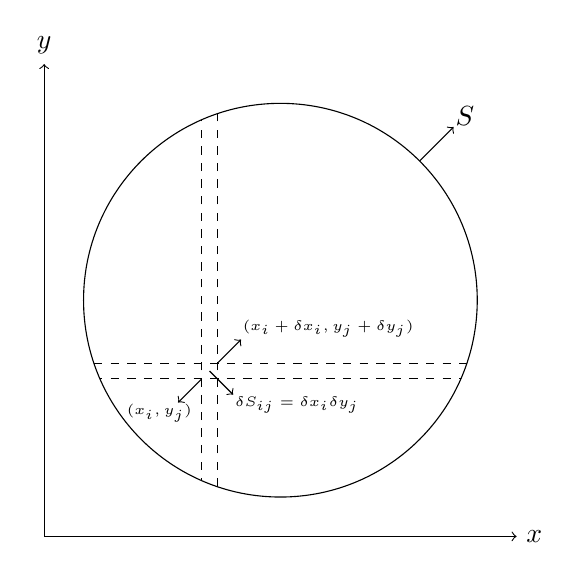
\begin{tikzpicture}
            \draw[<->] (0, 6) -- (0, 0) -- (6, 0);
            \node[above] at (0, 6) {\(y\)};
            \node[right] at (6, 0) {\(x\)};
            \draw (3, 3) circle (2.5cm);
            \begin{scope}
                \clip (3, 3) circle (2.5cm);
                \draw[dashed] (2, 0) -- (2, 6);
                \draw[dashed] (2.2, 0) -- (2.2, 6);
                \draw[dashed] (0, 2) -- (6, 2);
                \draw[dashed] (0, 2.2) -- (6, 2.2);
            \end{scope}
            \draw[->] (4.77, 4.77) -- (5.2, 5.2);
            \node[above right] at (5.1, 5.1) {\(S\)};
            \draw[->] (2.2, 2.2) -- (2.5, 2.5);
            \node[above right] at (2.4, 2.4) {{\tiny\((x_i + \delta x_i, y_j + \delta y_j)\)}};
            \draw[->] (2, 2) -- (1.7, 1.7);
            \node[below left] at (2, 1.8) {{\tiny\((x_i, y_j)\)}};
            \draw[->] (2.1, 2.1) -- (2.4, 1.8);
            \node[below right] at (2.3, 1.9) {{\tiny\(\delta S_{ij} = \delta x_i\delta y_j\)}};
        \end{tikzpicture}
        \caption{Integrating \(f(x, y)\)}
    \end{figure}
    The (Riemann) integral of \(f(x, y)\) for \(x, y\in S\) is defined as splitting area \(S\) into \(n\) vertical slices at positions \(x_i\) where \(x_i < x_{i + 1}\) and \(n\) horizontal slices at positions \(y_j\) where \(y_j < y_{j + 1}\).
    The width of the \(i^\text{th}\) vertical slice is \(\delta x_i\) and the width of the \(j^\text{th}\) horizontal slice is \(\delta y_j\).
    The area of the segment where \(x\in[x_i, x_{i + 1}]\) and \(y\in[y_j, y_{j + 1}]\) is then \(\delta S_{ij} = \delta x_i\delta y_j\).
    The integral is then found by summing up \(f\) evaluated at \((x_i, y_j)\) times the area of the segment as \(n\to \infty\) and \(\delta S_{ij}\to 0\).
    This gives
    \[I = \lim_{n\to \infty}\sum_{i = 0}^{n}\sum_{j=0}^n f(x_i, y_j)\delta S_{ij} = \int_S f(x, y)\,dS\]
    To avoid confusion later we also introduce the notation that the order of the \(f(x, y)\) and \(dS\) does not matter so the following are equivalent:
    \[\int_S f(x, y)\, dS = \int_S dS f(x, y)\]
    This integral can be interpreted as the volume between the surface and the \(x, y\) plane if and only if \(f(x, y)\) can be interpreted as the height above the \(x, y\) plane.
    Even then it is still a signed area (area below the \(x, y\) plane axis is negative).
    
    \subsection{Evaluating 2D Integrals}
    \begin{figure}[ht]
        \centering
        \begin{tikzpicture}
            \draw[<->] (3, 0) -- (0, 0) -- (0, 3);
            \node[right] at (3, 0) {\(x\)};
            \node[above] at (0, 3) {\(y\)};
            \draw (0.5, 2.5) rectangle (2.5, 0.5);
            \draw[dashed] (0, 2.5) -- (0.5, 2.5);
            \draw[dashed] (0, 0.5) -- (0.5, 0.5);
            \draw[dashed] (2.5, 0) -- (2.5, 0.5);
            \draw[dashed] (0.5, 0) -- (0.5, 0.5);
            \node[below] at (0.5, 0) {\(a\)};
            \node[below] at (2.5, 0) {\(b\)};
            \node[left] at (0, 0.5) {\(c\)};
            \node[left] at (0, 2.5) {\(d\)};
        \end{tikzpicture}
        \caption{A simple 2D integral}
        \label{fig:simple 2D integral}
    \end{figure}
    How do we evaluate a two dimensional integral?
    As an example we will integrate the function \(f\) over the area shown in figure \ref{fig:simple 2D integral}
    We can think of this being a 4 step process:
    \begin{enumerate}
        \item Increase \(x\) from \(a\) to \(b\) in steps of \(dx\) so \(a\to a + dx\to a + 2dx \to \dotsb\to b - dx\to b\)
        \item For each \(x\) value from step one increase \(y\) from \(c\) to \(d\) in steps of \(dy\) so \(c \to c + dy \to c + 2dy \to \dotsb \to d - dy\to d\)
        \item At each \((x, y)\) from steps one and two evaluate \(f(x, y)dxdy\)
        \item The integral is the sum of every result from step 3
    \end{enumerate}
    If we do the above for \(dx, dy\to 0\) then this is the integral.
    We can approximate the integral using non-zero \(dx\) and \(dy\) with the following C\hspace{-.05em}\raisebox{.4ex}{\tiny\textbf{++}} code:
    \begin{lstlisting}[language=C++]
        double f(double x, double y) {
            ...
        }
        
        double dx = 0.001;
        double dy = 0.001;
        double a = 1;
        double b = 2;
        double c = 1;
        double d = 2;
        
        double integral = 0;
        for (double x = 0; x < b; x += dx) {
            for (double y = 0; y < d; y += dy) {
               integral += f(x, y)  * dx * dy;
            }
        }
    \end{lstlisting}
    We can write this process with integrals as:
    \[\int_a^b dx\int_c^d dy\, f(x, y) \equiv \int_S dS\, f(x, y)\]
    The first integral written represents step one, the second integral written represents step two and the evaluation and summing in steps three and four are implicit in integrals.
    This is also written sometimes as the following:
    \[\int_a^b \int_c^d f(x, y) \,dy\,dx = \int_a^b dx\int_c^d f(x, y)\, dy\equiv \int_S dS\, f(x, y)\]
    but the order of integration can be tricky to deduce from this especially since not everyone is consistent.
    This means that the first way of writing it is probably best.
    It is also possible to be explicit in the limits about the variable for example replacing the \(a\) in the integral with respect to \(x\) with \(x = a\) this gives the most explicit (and maybe slightly pedantic) way of writing this as
    \[\int_{x = a}^{x = b} dx\int_{y = c}^{y = d} dy\, f(x, y) \equiv \int_S dS\, f(x, y)\]
    This is especially important when the limits aren't constants.
    
    \example
    \begin{align*}
        I &= \int_{x = 0}^3 dx\int_{y = 0}^4 dy\, xy\\
        &= \int_{x = 0}^3 dx\,x\left[\frac{y^2}{2}\right]_0^4\\
        &= \int_{x = 0}^3 dx\,8x\\
        &= 36
    \end{align*}
    We can take any variable that we aren't integrating with respect to as a constant.
    For constant limits \(a\), \(b\), \(c\) and \(d\) and functions \(g\) and \(h\) it is possible to do a separation of variables:
    \[\int_a^b dx\int_c^d dy\, g(x)h(y) = \left[\int_a^b g(x)\, dx\right]\left[\int_c^d h(y)\, dy\right]\]
    
    An example where this isn't possible is integrating over the triangle between the \(x\) axis, the line \(x = a\) and the line \(y = x\) for some function \(f\).
    If we split the triangle in the \(x\) direction first and then in the \(y\) direction we end up with slices of height \(y_i = x_i\) split into sections in the \(y\) direction.
    This results in the integral
    \[I = \int_0^a dx\int_0^x dy\, f(x, y)\]
    If instead we split the triangle in the \(y\) direction first and then in the \(x\) direction we get slices of length \(x_i = y_i\) split into sections in the \(x\) direction.
    This results in the integral
    \[I = \int_0^a dy\int_y^a dx\,f(x, y)\]
    \begin{figure}[ht]
        \centering
        \begin{tikzpicture}
            \draw[<->] (3, 0) -- (0, 0) -- (0, 3);
            \node[right] at (3, 0) {\(x\)};
            \node[above] at (0, 3) {\(y\)};
            \draw (0, 0) -- (3, 3);
            \draw[dotted] (2.5, 0) -- (2.5, 2.5);
            \node[below] at (2.5, 0) {\(a\)};
            \draw[lightgray] (1.3, 0) -- (1.3, 1.3);
            \draw[lightgray] (1.6, 0) -- (1.6, 1.6);
            \node[below] at (1.3, 0) {\(x_i\)};
            \foreach \x in {0.1, 0.2, ..., 1.3} {
                \draw[lightgray] (1.3, \x) -- (1.6, \x);
            }
            \foreach \x in {1.3, 1.4, 1.5} {
                \draw[lightgray] (\x, \x) -- (1.6, \x);
            }
            
            \begin{scope}[xshift=5cm]
                \draw[<->] (3, 0) -- (0, 0) -- (0, 3);
                \node[right] at (3, 0) {\(x\)};
                \node[above] at (0, 3) {\(y\)};
                \draw (0, 0) -- (3, 3);
                \draw[dotted] (2.5, 0) -- (2.5, 2.5);
                \node[below] at (2.5, 0) {\(a\)};
            \end{scope}
            \draw[lightgray] (6, 1) -- (7.5, 1);
            \draw[lightgray] (6.3, 1.3) -- (7.5, 1.3);
            \draw[dotted] (6, 1) -- (5, 1) node[left] at (5, 1) {\(y_i\)};
            \foreach \x in {6.3, 6.4, ..., 7.5} {
                \draw[lightgray] (\x, 1) -- (\x, 1.3);
            }
            \foreach \x in {6.1, 6.2} {
                \draw[lightgray] (\x, 1) -- ($(0, -5)+(\x, \x)$);
            }
        \end{tikzpicture}
        \caption{Splitting the same shape multiple ways}
    \end{figure}
    
    \example
    \begin{align*}
        I &= \int_1^2 dx\int_x^2 dy\,\frac{1}{y}\\
        &= \int_1^2 dx\,[\ln y]_x^2\\
        &= \int_1^2 dx\,[\ln 2 - \ln x]\\
        &= [x\ln 2 - x\ln x + x]_1^2\\
        &= 2\ln 2 - 2\ln 2 + 2 - (\ln 2 - \ln 1 + 1)\\
        &= 2 - \ln 2 - 1\\
        &= 1 - \ln 2
    \end{align*}
    This integral can be calculated much more easily by swapping the order of integration
    \begin{align*}
        I &= \int_1^2 dx\int_x^2 dy\,\frac{1}{y}\\
        &= \int_1^2 dy\int_1^y dx\, \frac{1}{y}\\
        \intertext{The integral with respect to \(x\) must be calculated first as its limits depend on \(y\)}
        &= \left[\int_1^2 dy\frac{1}{y} \right]\left[ \int_1^y dx\right]\\
        &= \int_1^2 dy\,[x]_1^y\\
        &= \int_1^2 dy\,\frac{1}{y}(y - 1)\\
        &= \int_1^2 dy \left[1 - \frac{1}{y}\right]\\
        &= [y - \ln y]_1^2\\
        &= 2 - \ln 2 - (1 - \ln 1)\\
        &= 1 - \ln 2
    \end{align*}
    The second way round avoids having to integrate \(\ln x\).
    When swapping the order of integration one must take care to ensure that the limits of the integrals are correct.
    
    \example
    \[I = \int_0^1 dx\int_0^{2 - x}dy\,\frac{x}{y}\]
    (Note that this integral is actually undefined as \(x/y\) can't be evaluated at \(y = 0\))
    This is asking us to integrate over the region \(R\) in figure \ref{fig:region of integration}.
    The way the integral is written the integral with respect to \(y\) is calculated first.
    If we want to swap the order of the integrals we need to consider that depending on the value of \(y\) the equation of the line bounding the space changes.
    This means that we have to split the integral at the intersection.
    \begin{figure}[ht]
        \centering
        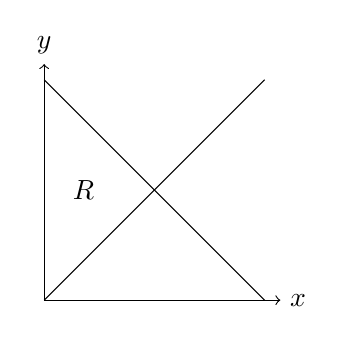
\begin{tikzpicture}
            \draw[<->] (3, 0) -- (0, 0) -- (0, 3);
            \node[right] at (3, 0) {\(x\)};
            \node[above] at (0, 3) {\(y\)};
            \draw (0, 0) -- (2.8, 2.8);
            \draw (2.8, 0) -- (0, 2.8);
            \node at (0.5, 1.4) {\(R\)};
        \end{tikzpicture}
        \caption{Region bounded by \(x = 0\), \(y = x\) and \(y = 2 - x\)}
        \label{fig:region of integration}
    \end{figure}
    The limits go from \(y\to x\) and \(y = 2 - x\to x = 2 - y\).
    \[I = \left[\int_0^1dy\int_0^ydx\,\frac{x}{y}\right] + \left[\int_1^2dy\int_0^{2 - y}dx\,\frac{x}{y}\right]\]
    This is now separable as
    \[I = \left[\int_0^1 dy\,\frac{1}{y}\int_0^ydx\,x\right] + \left[\int_1^2 dy\,\frac{1}{y}\int_0^{2-y}dx\, x\right]\]
    This technique can make undoable (in elementary functions) integrals possible, for example the integral
    \[I = \int_0^1 dy\int_y^1 dx\,\frac{\sin x}{x}\]
    is impossible to do in elementary functions but by swapping the order of integration we get
    \begin{align*}
        I &= \int_0^1 dx\int_0^x dy\,\frac{\sin x}{x}\\
        &= \int_0^1 \left[\frac{\sin x}{x}y\right]_0^x\,dx\\
        &= \int_0^1 \sin x\,dx\\
        &= [-\cos x]_0^1\\
        &= 1 - \cos 1
    \end{align*}
    
    \section{Change of Basis}
    \subsection{Polar Coordinates}
    If we want to integrate over the surface \(S\) that is a circle radius \(R\) centre \((0, 0)\) then we \emph{can} do this in Cartesian coordinates.
    If we first split the surface in to strips in the \(x\) direction then this gives us \(x\) limits of \(-R\) and \(R\).
    We next split the each strip in the \(y\) direction.
    This gives \(y\) limits of \(y = \pm\sqrt{R^2 - x^2}\) since the equation of the circle is \(x^2 + y^2 = R^2\).
    Therefore the integral of the function \(f\) over \(S\) is
    \[I = \int_S dS\,f(x, y) = \int_{-R}^R dx\int_{-\sqrt{R^2 - x^2}}^{\sqrt{R^2 - x^2}} dy\,f(x, y)\]
    however the limits make this horrible even before we consider what \(f(x, y)\) is.
    
    It is easier to calculate this integral in polar coordinates which are related to Cartesian coordinates by:
    \[x = \rho\cos\varphi\qquad y = \rho\sin\varphi\]
    To do this we split the circle as shown in figure \ref{fig:integrating over a circle}.
    \begin{figure}[ht]
        \centering
        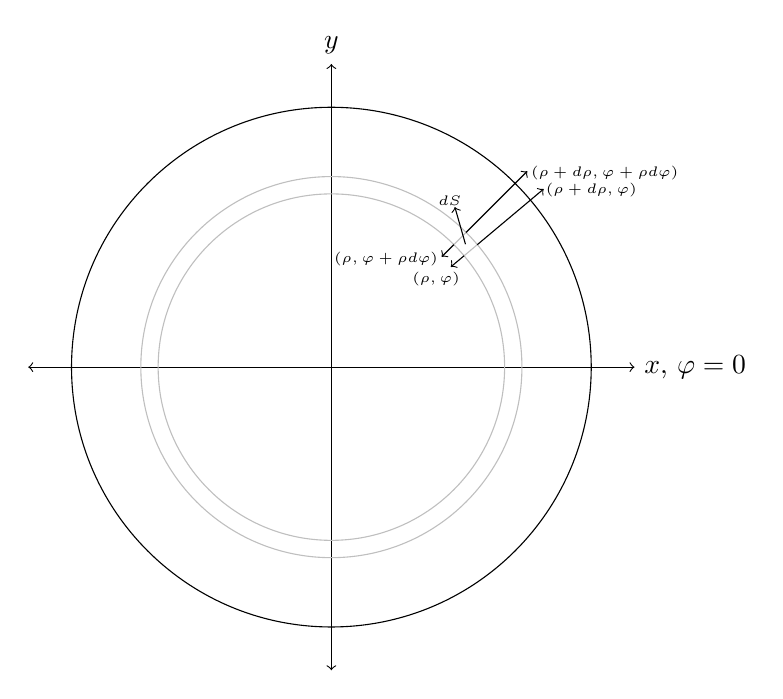
\begin{tikzpicture}[xscale=1.1, yscale=1.1]
            \draw[<->] (-3.5, 0) -- (3.5, 0) node[right] at (3.5, 0) {\(x\), \(\varphi = 0\)};
            \draw[<->] (0, -3.5) -- (0, 3.5) node[above] at (0, 3.5) {\(y\)};
            \draw (0, 0) circle (3cm);
            \draw[lightgray] (0, 0) circle (2cm);
            \draw[lightgray] (0, 0) circle (2.2cm);
            \begin{scope}[rotate=40]
                \draw[lightgray] (2, 0) -- (2.2, 0);
                \draw[->] (2.2, 0) -- (3.2, 0);
                \draw[->] (2, 0) -- (1.8, 0);
                \node[above right] at (3, -0.1) {{\tiny\((\rho + d\rho, \varphi)\)}};
                \node[below left] at (2, -0.1) {{\tiny\((\rho, \varphi)\)}};
            \end{scope}
            \begin{scope}[rotate=45]
                \draw[lightgray] (2, 0) -- (2.2, 0);
                \draw[->] (2.2, 0) -- (3.2, 0);
                \draw[->] (2, 0) -- (1.8, 0);
                \node[above right] at (3, -0.1) {{\tiny\((\rho + d\rho, \varphi + \rho d\varphi)\)}};
                \node[above left] at (1.7, -0.2) {{\tiny\((\rho, \varphi + \rho d\varphi)\)}};
            \end{scope}
            \begin{scope}[rotate=42.5]
                \draw[->] (2.1, 0) -- (2.3, 0.4);
                \node[above left] at (2.37, 0.2) {{\tiny\(dS\)}};
            \end{scope}
        \end{tikzpicture}
        \caption{Integrating over a circle}
        \label{fig:integrating over a circle}
    \end{figure}
    The area \(dS\) tends to a rectangle as \(d\rho\to 0\).
    This rectangle has side lengths \(d\rho\) and \(\rho d\varphi\) so the area is given by \(dS = dx\,dy = \rho\,d\rho\,d\varphi\).
    This circle has \(\rho\) limits \(0\) to \(R\) and \(\varphi\) limits \(0\) to \(2\pi\).
    This means our integral \(I\) is
    \[I = \int_0^R d\rho\int_0^{2\pi}d\varphi \rho f(x, y)\]
    \example
    \begin{align*}
        I &= \int dS\, xy\\
        &= \int_0^Rd\rho\int_0^{2\pi}d\varphi\,\rho\rho\cos\varphi\rho\sin\varphi\\
        &= \int_0^Rd\rho\int_0^{2\pi}d\varphi\,\rho^3\cos\varphi\sin\varpi\\
        &= \left[\int_0^R\rho^3\,d\rho\right]\left[\in_0^{2\pi}\cos\varphi\sin\varphi\,d\varphi\right]\\
        &= \left[\frac{\rho^4}{4}\right]_0^R\left[\frac{1}{2}\sin^2\varphi\right]_0^{2\pi}\\
        &= 0
    \end{align*}
    The fact that this is 0 makes sense since the surface is symmetric about both axis and the function will be negative in top left and bottom right quadrants and positive elsewhere so much like an odd function integrated over even limits the positive and negative parts cancel to 0.
    
    \subsection{The Jacobian}
    It was (relatively) easy to work out that \(dx\,dy = \rho d\rho\,d\varphi\) geometrically but this will not always be the case, especially in higher dimensions.
    We want to come up with a method for working out the element we integrate in the general case.
    
    Consider two coordinate systems the Cartesian \((x, y)\) system and some irregular \((u, v)\) system.
    Let \(\vv a\) be a vector along a line of constant \(v\) and \(\vv b\) be a vector along a line of constant \(u\).
    We can work out what \(\vv a\) and \(\vv b\) are in terms of \(\vv x\) and \(\vv y\) which are vectors in the \(x\) and \(y\) directions respectively and \(du\) and \(dv\) which are small displacements in the \(u\) and \(v\) directions respectively
    \[\vv a = \pdv{x}{u} du\vv x + \pdv{y}{u}du\vv y\]
    \[\vv b = \pdv{x}{v}dv\vv x + \pdv{y}{v}dv\vv y\]
    We can put \(\vv a\) and \(\vv b\) as the columns of a matrix and make this a matrix equation using the fact that a determinant is a scale factor for the transformation we can get \(dS\):
    \[
        dS = dx\,dy = \left |\det
        \begin{pmatrix}
            \pdv{x}{u}du & \pdv{x}{v}dv \\
            \pdv{y}{u}du & \pdv{y}{v}dv
        \end{pmatrix}
        \right |
    \]
    \[= \left |\pdv{x}{u}du\pdv{y}{v}dv - \pdv{x}{v}dv\pdv{y}{u}du\right |\]
    \[= \left |\pdv{x}{u}\pdv{y}{v} - \pdv{x}{v}\pdv{y}{u}\right |du\,dv\]
    \[
        = \left |\det
        \begin{pmatrix}
            \pdv{x}{u} & \pdv{x}{v} \\
            \pdv{y}{u} & \pdv{y}{v}
        \end{pmatrix}
        \right |du\,dv
    \]
    The matrix in the last step is the Jacobian matrix (often just the Jacobian) change of basis. The (absolute value of the) determinant is then known as the Jacobian derivative (confusingly also often just the Jacobian).
    In general the Jacobian takes in two \(n\) and \(m\) dimensional sets of coordinates \(x_i\) and \(x_j'\) and gives the relationship between the unit volumes.
    There are various notations for the Jacobian, some of these are
    \[J = J(x_1', x_2', \dotsc, x_n') = \pdv{(x_1, x_2, \dotsc, x_m)}{(x_1', x_2', \dotsc, x_n')}\]
    The \(n\times m\) Jacobian matrix is then defined by
    \[J_{ij} = \pdv{x_i}{x_j'}\]
    A few shortcuts with determinants are useful here, for an \(n\times n\) matrix \(M\):
    \begin{itemize}
        \item \(\det(M) = \det(M\trans)\) so if you accidentally calculate \(\pdv{x_i'}{x_j}\) instead for \(J_{ij}\) it doesn't matter
        \item A transformation \(M\to M'\) that results in one row or column being multiplied by \(k\) has determinant \(\det(M') = k\det(M)\)
        \item Multiplication of \(M\) by a scalar \(k\) results in a determinant \(\det(kM) = k^n\det(M)\).
        This can be thought of as each row individually being multiplied by \(k\).
    \end{itemize}
    
    \subsection{Cylindrical Coordinates}
    Cylindrical coordinates are related to Cartesian coordinates by
    \[x = \rho\cos\varphi \qquad y = \rho\sin\varphi \qquad z = z\]
    If we are going to integrate over a cylinder radius \(R\) height \(h\) placed such that \(z = 0\) is halfway up the cylinder then the \(\rho\) limits are 0 and \(R\), the \(\varphi\) limits are 0 and \(2\pi\) and the \(z\) limits are \(-h/2\) and \(h/2\).
    The Jacobian is
    \[
        \pdv{(x, y, z)}{(\rho, \varphi, z)} = \left | \det
        \begin{pmatrix}
            \cos\varphi & \sin\varphi & 0 \\
            -\rho\sin\varphi & \rho\cos\varphi & 0\\
            0 & 0 & 1
        \end{pmatrix}
        \right |
    \]
    \[= |\cos\varphi\rho\cos\varphi + \rho\sin\varphi\sin\varphi|\]
    \[= \rho\]
    Hence a volume element \(dV\) is
    \[dV = dx\,dy\,dz = \rho d\rho\,d\varphi\, dz\]
    Hence an integral over a cylinder can be calculated as
    \[\int_V dV f(x, y, z) = \int_0^R d\rho \int_0^{2\pi} d\varphi \int_{-h/2}^{h/2}dz\, \rho f(\rho\cos\varphi, \rho\sin\varphi, z)\]
    Note that the limits for \(z\) depend on the location of the origin.
    
    \section{Spherical Coordinates and the Laplacian}
    \subsection{Integrating in Spherical Coordinates}
    When trying to integrate over a spherically symmetric volume \(V\) it is best to do it in spherical coordinates.
    \[x = r\sin\vartheta\cos\varphi,\qquad y = r\sin\vartheta\sin\varphi,\qquad z = r\cos\vartheta\]
    where \(r \in [0, \infty)\) is the distance from the origin to the point, \(\varphi \in [0, 2\pi]\) is the angle from the \(x\) axis to the projection of the point in the \(x\), \(y\) plane and \(\vartheta \in [0, \pi]\) is the angle from the \(z\) axis to the line connecting the origin and the point.
    We need to calculate the value of the Jacobian for spherical coordinates:
    \begin{align*}
        J &= \pdv{(x, y, z)}{(r, \vartheta, \varphi)}\\
        &= \left | \det
        \begin{pmatrix}
            \sin\vartheta\cos\varphi & \sin\vartheta\sin\varphi & \cos\vartheta\\
            r\cos\vartheta\cos\varphi & r\cos\vartheta\sin\vartheta & -r\sin\vartheta\\
            -r\sin\vartheta\sin\varphi & r\sin\vartheta\cos\vartheta & 0
        \end{pmatrix}
        \right |\\
        & = | \cos\vartheta(r^2\cos\vartheta\sin\vartheta\cos^2\varphi + r^2\cos\vartheta\sin\vartheta\sin^2\varphi) \\
        &\hphantom{=|} + r\sin\vartheta (r\sin^2\vartheta\cos^2\varphi + r\sin^2\vartheta\sin^2\varphi)|\\
        & = |r^2\cos^2\vartheta\sin\vartheta + r^2\sin^2\vartheta\sin\vartheta|\\
        & = r^2\sin\vartheta
    \end{align*}
    since \(\vartheta\in[0, \pi]\) \(\sin\vartheta \ge 0\A \vartheta\).
    This means that a volume element \(dV\) is given by
    \[dV = dx\,dy\,dz = r^2\sin\vartheta,dr\,d\vartheta\,d\varphi\]
    Hence the integral of a function \(f\) over all space is given by
    \[\int_V dV = \int_{-\infty}^\infty dx \int_{-\infty}^\infty dy \int_{-\infty}^\infty dz\,f(x, y, z) = \int_0^\infty dr\int_0^\pi d\vartheta\int_0^{2\pi} d\varphi\, f(r\sin\vartheta\cos\varphi, r\sin\vartheta\sin\varphi, r\cos\vartheta)\]
    
    \subsection{The Laplacian}
    On page \pageref{sec:grad} section \ref{sec:grad} we defined the gradient operator \(\grad\) as a vector of partial derivatives
    \[\grad_i = \pdv{x_i}\]
    another useful operator is it turns out this dotted with itself, in \(n\) dimensions this is:
    \[\grad\cdot\grad = \laplacian = \sum_{i = 1}^{n} \pdv[2]{x_i}\]
    For example in 3 dimensions:
    \[\laplacian = \pdv[2]{x} + \pdv[2]{y} + \pdv[2]{z}\]
    This is very common in physics for example in the Schr\"odinger equation:
    \[-\frac{\hbar^2}{2m}\laplacian \psi(\vv r, t) + V(\vv r, t) = i\hbar \pdv{t}\psi(\vv r, t)\]
    or the in the wave equation:
    \[\pdv[2]{u}{t} = c^2\laplacian u\]
    It is also possible to write these operators in polar coordinates of some kind.
    To do this we find the derivative of some arbitrary function \(f\) with respect to our new basis coordinates (\(\rho\), \(r\), \(\varphi\),\(\vartheta\), whatever else we are using) and set up and solve simultaneous equations for the differential operators with respect to our initial base (\(x\), \(y\), \(z\) etc.) and then we apply these to themselves to find the second derivatives.
    For example in plane polar coordinates:
    \[x = r\cos\varphi,\qquad y = r\sin\varphi\]
    \[\laplacian = \pdv[2]{x} + \pdv[2]{y}\]
    \begin{align*}
        \pdv{f}{\rho} &= \pdv{x}{\rho}\pdv{f}{x} + \pdv{y}{\rho}\pdv{f}{y}\\
        &= \cos\varphi\pdv{f}{x} + \sin\varphi\pdv{f}{y}\\
        \pdv{\rho} &= cos\varphi\pdv{x} + \sin\varphi\pdv{y}\stepcounter{equation}\tag{\theequation}\label{eqn:diff wrt rho}\\
        \pdv{f}{\varphi} &= \pdv{x}{\varphi}\pdv{f}{x} + \pdv{y}{\varphi}\pdv{f}{y}\\
        &= -\rho\sin\varphi \pdv{f}{x} + \rho\cos\varphi\pdv{f}{y}\\
        \pdv{\varphi} &= -\rho\sin\varphi \pdv{x} + \rho\cos\varphi\pdv{y}\stepcounter{equation}\tag{\theequation}\label{eqn:diff wrt phi}
    \end{align*}
    We can solve the simultaneous equations \ref{eqn:diff wrt rho} and \ref{eqn:diff wrt phi} to get our differential for \(x\) and \(y\).
    Doing this gives us
    \begin{align*}
        \pdv{x} &= \cos\varphi\pdv{\rho} - \frac{\sin\varphi}{\rho}\pdv{\varphi}\\
        \pdv{y} &= \sin\varphi\pdv{\rho} + \frac{\cos\varphi}{\rho}\pdv{\varphi}
    \end{align*}
    Finally we can calculate the Laplacian as
    \begin{align*}
        \laplacian &= \pdv[2]{x} + \pdv[2]{y}\\
        &= \left[\cos\varphi\pdv{\rho} - \frac{\sin\varphi}{\rho}\pdv{\varphi}\right]\left[\cos\varphi\pdv{\rho} - \frac{\sin\varphi}{\rho}\pdv{\varphi}\right]\\
        &\hphantom{=|} + \left[\sin\varphi\pdv{\rho} + \frac{\cos\varphi}{\rho}\pdv{\varphi}\right]\left[\sin\varphi\pdv{\rho} + \frac{\cos\varphi}{\rho}\pdv{\varphi}\right]\\
        &= \frac{1}{\rho}\pdv{\rho}\left(\rho\pdv{\rho}\right) + \frac{1}{\rho}\pdv{\rho} + \frac{1}{\rho^2}\pdv[2]{\varphi}\\
        &= \pdv[2]{\rho} + \frac{1}{\rho}\pdv{\rho} + \frac{1}{\rho^2}\pdv[2]{\varphi}
    \end{align*}
    Following the same method it is possible to derive the Laplacian in cylindrical and spherical coordinates as well.
    Cylindrical:
    \[\laplacian = \frac{1}{\rho} \pdv{\rho} \left(\rho\pdv{\rho}\right) + \frac{1}{\rho^2} \pdv[2]{\varphi} + \pdv[2]{z}\]
    Spherical:
    \[\laplacian = \frac{1}{r^2}\pdv{r}\left(r^2\pdv{r}\right) + \frac{1}{r^2\sin\vartheta} \pdv{\vartheta} \left(\sin\vartheta\pdv{\vartheta}\right) + \frac{1}{r^2\sin^2\vartheta}\pdv[2]{\varphi}\]
\end{document}
